% -------------------------------------------------------------------------------------------------
%
%  Skeleton for theses at the Institute of Robotics and Intelligent Systems
%
% -------------------------------------------------------------------------------------------------
%
% FILENAME:   thesis.tex
%
% ABSTRACT:   main file for theses
%
% EXCEPTIONS: -
%
% USAGE:      !!!!!!COMPILE WITH PDFLATEX, *NOT* WITH LATEX OR TEX!!!!!!!
%
% HISTORY:    written by Sascha A. Stoeter <stoeter@iris.ethz.ch>, www.stoeter.com, 02.06.2004
%             modified by Martin Probst, 18.08.2004
%             modified by Chauncey Graetzel, 11.05.2005

% -------------------------------------------------------------------------------------------------

\documentclass[12pt,a4paper,onecolumn]{article}
\usepackage{irisarticle}

% -------------------------------------------------------------------------------------------------
% Add needed packages. Some generally useful packages are listed for
% your convenience.
% -------------------------------------------------------------------------------------------------
\usepackage{subfigure}                          % enable the use of subfigures
%\usepackage[bf]{caption}                       % must go after subfigure
\usepackage[thickspace,thinqspace]{SIunits}     %

\usepackage{hyperref}                           % enable Hyperlinks in pdf/ps Docs
\usepackage{pdfpages}



% -------------------------------------------------------------------------------------------------
% Some handy definition to simplify future markup changes
% -------------------------------------------------------------------------------------------------
\providecommand{\eg}{e.g.}
\providecommand{\etal}{\textit{et al.}}
\providecommand{\ie}{i.e.}

%\setlength{\textwidth}{18cm} \setlength{\oddsidemargin}{-1cm}
%\setlength{\evensidemargin}{-1cm}

% -------------------------------------------------------------------------------------------------
% Select type of thesis
% -------------------------------------------------------------------------------------------------
\renewcommand{\iristhesistype}{Bachelor}

% -------------------------------------------------------------------------------------------------
% Set names
% -------------------------------------------------------------------------------------------------
\renewcommand{\irisauthor}{Berk Nergiz}
%:
\renewcommand{\irisadviser}{}


% -------------------------------------------------------------------------------------------------
% Beginning of the main document body
% -------------------------------------------------------------------------------------------------
\begin{document}

% include all Bib-items even if they're not cited in the text
\nocite{*}

% This is the first part of the front matter. Pages appear unnumbered
% and the pages are not counted.

% Title page: set title and date preferably formatted according to
% ISO 8601
\iristitlepage{1D Computations of Flow and Oxygen Transport in Micro-Vascular Networks}{June 2018}


% This is the second part of the front matter. Pages appear with
% lowercase roman numbering. The first page number is 'i'.
\pagenumbering{roman}

% Table of contents
\newpage
\tableofcontents
\addtocontents{toc}{\vspace{.5\baselineskip}}

% List of tables
%\newpage
%\addcontentsline{toc}{section}{\protect\numberline{}{List of Tables}}
%\listoftables

% List of figures
%\newpage
%\addcontentsline{toc}{section}{\protect\numberline{}{List of Figures}}
%\listoffigures

\clearpage
\pagenumbering{arabic}

% This is the main part of the thesis. Pages appear with arabic numbering.

% Abstract must not be longer than one page per language.
\addcontentsline{toc}{section}{\protect\numberline{}{Abstract}}
\markright{Abstract}
\section*{Abstract}

Oxygen is carried by red blood cells in the blood. It is supplied to organs, muscles and generally to the tissue through complex networks. This microvascular network consists of micro-sized capillaries, that can be extracted from ex vivo mice organs. This work is part of the NCCR Kidney project, and aimed to develop and analyze computational models to understand the gradients of Oxygen in the tissue, and have a better understanding of what methods might be the most accurate ones in order to get physiologically correct results.

% Main body
% \section{Introduction}
\label{s:Introduction}

\subsection{Motivation}

This thesis aims to understand and specify how blood flow and oxygen transport has been simulated until today. The goal is to see how far existing methods, especially the Greens' Method developed by Secomb et. al can produce accurate results, and differentiate between different networks. A new model using an open source software called DuMuX was implemented to offer a different approach for oxygen transport and diffusion simulations.

\subsection{Structure of Thesis}

This thesis will have following structure ...

%!TEX root = article.tex

\section{Introduction}
\label{s:Introduction}

\subsection{Motivation}
%Why do we do this at all ?

This thesis aims to understand and specify how blood flow and oxygen transport has been simulated until today. The goal is to see how far existing methods, especially the Green's Function Method applied to this field by Secomb et al. \cite{Secomb2004} can produce accurate results for new and especially complex networks. A new model using an open source software called $DuMu^x$ was implemented to offer a different approach for oxygen transport and diffusion simulations.

\subsection{Structure of the Thesis}
%This thesis will have following structure ...

First, a short inside to the physiological background of blood flow and oxygen transport in the body and especially to the tissue will be given. Linked to this, the main subject will be the transport of oxygen in the body, starting in the blood flow and ending in the diffusion into the tissue through a general diffusion process.
\\The results of oxygen transport simulation methods, especially the Green's Function Method, was evaluated using different networks. In addition to this, a new oxygen delivery model was implemented using an open source software called $DuMu^x$. The focus of this thesis is to understand when and why the Green's Function Method produces physiologically accurate results, how it can perform on new networks and compare these results to alternatives such as the implemented method on $DuMu^x$.

\section{Blood Flow and Oxygen Delivery}
%How does this work physiologically ?

In this section the physiological aspects will be discussed, and the main goal of computations and simulations in this field will be explained. This part is mainly about the physiological points in blood flow and oxygen transport, as well as oxygen consumption in tissue and further outlook in this field (i.e. EPO and tumor oxygen delivery etc.)

\subsection{Blood Flow}
%Purely physiological Blood Flow part (with mathematical formulas to describe processes)

Blood flow in the body can be approximated by the Navier-Stokes equations.
\\But rather talk about purely physiological things first.
\\Put some papers and references in and explain some values and parameters.
\\Use mathematics paper for blood flow calculations

\subsection{Oxygen Transport and Delivery}
%Purely physiological Oxygen part (with mathematical formulas to describe processes)

How does this physically and physiologically work ?
\\Again put some papers and references in and explain some physical diffusion equations, values and parameters.
\\Why do we care about this etc. ?
\\Diffusion, Parameters, etc. etc.
\\Use Vasomotion paper for oxygen delivery

\subsection{Current Trends in Modeling}
%Use a few papers to give examples for previous and actual approaches

Do link to modeling and models in this field in general, than link this to computational models in this field and their use. Actual trends and what people hope for in the future (in terms of computational power, computational methods but also from a medical perspective) is also interesting.
\\Generally Blood Flow in the body can be approximated by the Navier-Stokes equations. The Transport of Oxygen in the Blood can then be linked to this by the Transport Equations. These physical equations are quite straightforward to implement and solve numerically. The next task remains the biggest problem in actual research: Link this transport to the diffusion process out of the vessels and into the tissue. The biggest problems here seem to be in choosing the right/appropriate boundary conditions to get exact results. Also, many numerical methods fail or more specifically become unstable when the vessel network becomes complicated and heterogeneous.

%In each of your categories (or subcategories if your topic is
%broad), we would like the following three points to be developed:
%\begin{enumerate}
 %   \item Concepts, definitions, value
%of this topic etc. For explanations that do not really fit in the
%text you may want to use footnotes\footnote{footnotes are shown
%below like this.} or by using the appendix (e.g. "see appendix
%\ref{s:ExtraStuff}").
 %   \item State of the art, discussing the work in the field, etc. E.g. Shaninpoor et al. \cite{shaninpoor98} have shown that ...
 %   \item Outlook: where do you feel this field is going. How would you continue your research on this
  %  topic?
%\end{enumerate}

\section{Simulation Methods}
%Everything about the computations behind the simulations and all I did.

As mentioned previously, this thesis is focussing on the analysis of simulation methods for oxygen transport and the delivery to tissue surrounding the vessels. In this section I will limit the analysis of simulation methods to the Green's Function Method and accordingly the code developed by Secomb et al. \cite{Secomb2004}, and a new model I implemented using $DuMu^x$. Both the methods and the produced results will be discussed in the following sections.

\subsection{Green's Function Method Code}
%Here I will talk about everything concerning the Green's Method Code.

The Green's Function Method was first used for numerical computations of Oxygen delivery in the tissue by Secomb et al. \cite{Secomb2004}. It can deliver accurate results with lower computational cost, due to the fact that the number of unknowns is reduced. For simple networks like the examples specified in the next chapter, the method seems to be stable and produce accurate results. However, using new and more complex networks, the Green's Function Method seems to produce bad results and shows characteristics of unstability (at least we think so for now). Obviously as the results get bad, the computational advantages of this method are not of any use (bad formulation?).
\\The mathematical background behind the Green's Function Method and the numerical method derived from it will be discussed in the upcoming section. The accuracy of produced results as well as the physiological meaning behind these results will be the main subject in this chapter.

\subsubsection{Green's Function Model}
%Just mathematical theory behind this method

General explanation about Green's Method code and how it works, especially mathematics behind the Green's Function Method (many mathematical formulas) and why it makes sense to use this. Also especially why is this interesting in physiological applications and oxygen delivery/consumption simulations ?
\\Goals:
\\- Avoid no flux boundary condition
\\- Find a systematic method that can be applied to tissue domains of arbitrary shape
\\- Find a cheap solution in terms of computational cost (when compared to implicit methods)
\\- Green's function method is computationally less expensive than implicit methods, due to the fact that there is a lower number of unknowns

\subsubsection*{Mathematics Behind Green's Function Method}
%Mathematical Background to this Method. What's so special about it ? Is there any advantage at first sight ?
%Very useful to use Green's Function Formulation section of Secomb here

This part strongly relies on the description by Secomb et al. \cite{Secomb2004}. In this subsection, the Green's Function Method, its equations and application to the given problem/field will be explained.
\\In this section, I will focus on giving a good and understandable insight to the Green's Function Method and its specific application, instead of getting lost in details. More specific low-level informations about the code and its implementation will follow later.
\\The main idea of the Green's Function Method approach is to model blood vessels as discrete Oxygen sources. This 
%Explain Equation and variables
\begin{equation}
\\D\alpha\nabla^2G = - \delta_3 
( \textbf{x} - \textbf{x*} )
\label{eq:Greens1}
\end{equation}
\ref{eq:Greens1} is obtained by putting G(\textbf{x}; \textbf{x*}) as the Green's Function, and saying that it is defined as the potential at \textbf{x} resulting from a source at \textbf{x*}.
%Explain Equation and variables
\begin{equation}
\textbf{P(x)} = \int_{Sources} G(\textbf{x; x*})q(\textbf{x*})d\textbf{x*}
\label{eq:Potential}
\end{equation}
\ref{eq:Potential} gives the potential, with q(x) representing the distribution of source strengths.
%Explain Equation and variables
\begin{equation}
\\G = G_1 = \frac{1}{(4 \Pi D \alpha |( \textbf{x} - \textbf{x*} )|)}
\label{eq:InfDomain}
\end{equation}
\ref{eq:InfDomain} gives the solution on an infinite domain, which is the singular function.
%Explain Equation and variables
\begin{equation}
\\q_v(s) = \int_{0}^L F(s-s^*)q_0(s^*)ds*
\label{eq:DiffFlux}
\end{equation}
\ref{eq:DiffFlux} gives the actual diffusive flux at the blood–tissue boundary.
\\The distribution of radial flux across the cylindrical surface is obtained by the function F(s), where s is the distance along the vessel.
%Explain Equation and variables
\begin{equation}
\\F(s) = \frac{1}{2} \delta_1 (s) + \frac{k (K(k) - E(k)}{4 \Pi r_0}
\label{eq:DiffFluxUni}
\end{equation}
\ref{eq:DiffFluxUni} for sources that are uniformly distributed around the circumference.
%Explain Equation and variables
\\Where K(k) \ref{eq:EllipInt1} and E(k) \ref{eq:EllipInt2} represent the complete elliptic integrals of the first and second kind respectively :
\begin{equation}
\\K(k) = \int_{0}^{\frac{\Pi}{2}} (1 - k^2 sin^2 \Theta)^ \frac{-1}{2} d \Theta
\label{eq:EllipInt1}
\end{equation}
%Explain Equation and variables
\begin{equation}
\\E(k) = \int_{0}^{\frac{\Pi}{2}} (1 - k^2 sin^2 \Theta)^ \frac{1}{2} d \Theta
\label{eq:EllipInt2}
\end{equation}


\subsubsection*{The Computational Model}
%Methods and physiological assumptions used in this model.
%Very useful to use Governing Equations section of Secomb here

In this subsection, the used physical quantities, the assumptions and governing equations will briefly be explained. The equations cited here are, in my opinion, the most important ones to describe the physical background for the treated problem. Similar to the previous section, this section will strongly rely on \cite{Secomb2004}.
\\When looking at the code of the Green's Function Method, and especially at the inputs \ref{Inputs}, one can see that the tissue is modeled as a homogeneous medium. This results in constant Oxygen diffusivity and solubility coefficients D and $\alpha$ respectively. These quantities usually have to be specified in the SoluteParams.dat-file. A more detailed explanation to the Inputs can be found in the Inputs section \ref{Inputs}.
\\The governing equations are listed here, with a short explanation for each of them:
\\As previously described, diffusion will play an important role in Oxygen transport in the body, as Oxygen is reaching the tissue by diffusing out of the vessels. This physical phenomenon is described by Fick's Law of Diffusion:
\begin{equation}
\\J = - D \frac{dc}{dx}
\label{Fick}
\end{equation}
%
Where J is the diffusive flux, D is the previously mentioned diffusivity coefficient, and dc/dx is the derivative of the concentration with respect to the distance x.
\\In addition to this, the principle of conservation of mass applies to Oxygen, and we have:
\begin{equation}
\frac{\delta \rho} {\delta t} + \nabla (\rho v) = 0
\end{equation}
%
These two fundamental equations can be combined to finally get:
\begin{equation}
\\D\alpha\nabla^2P = M(P)
\label{eq:DiffusionEq}
\end{equation}
%
\ref{eq:DiffusionEq} describes the dependency between the Oxygen partial pressure P and the consumption rate M(P). Here I would like to mention the fact that partial pressure is physically nothing else than the concentration used in \ref{Fick}.
For the consumption, a Michaelis-Menten relationship applied to the problem is used:
\begin{equation}
\\M(P) = \frac{M_0P}{(P_0 + P)}
\label{eq:MichaelisMenten}
\end{equation}
%
In \ref{eq:MichaelisMenten}, M(P) is the consumption, $M_0$ the demand and $P_0$ the partial pressure at half-maximal consumption.
\\As previously mentioned, the second important physical phenomenon to describe our transport problem is the convective transport in the blood flow. To model this, we need to know the rate of convective Oxygen that is transported through a single vessel segment.
\begin{equation}
\\f(P_b) = Q(H_DC_0S(P_b) + \alpha_{eff}P_b)
\label{eq:ConvTrans}
\end{equation}
%
In \ref{eq:ConvTrans}, the flow rate of blood is Q, and $H_D$, S, $C_0$, $P_b$ and $\alpha_{eff}$ are parameters such as discharge hematocrit, oxyhemoglobin saturation or partial pressure of oxygen in the blood. (Here specify everything yes or no ? Maybe use a symbols table at beginning to make things easier).
\\The previously mentioned oxyhemoglobin saturation can be computed by Hill's equation:
\begin{equation}
\\S(P_b) = \frac{P_b^n}{(P_b^n+P_{50}^n)}
\label{eq:Hill}
\end{equation}
In Hill's equation \ref{eq:Hill}, $P_b$ ist the previously mentioned partial pressure of oxygen in blood, $P_{50}$ is the partial pressure of oxygen at 50\% saturation and n is a constant.
%
\\Another important equation that we need to describe the given problem is the relationship describing the rate of of diffusive oxygen efflux per unit vessel length:
\begin{equation}
\\ \frac{df(P_b)}{ds} = -q_v(s)
\label{eq:ConsOxygen}
\end{equation}
\ref{eq:ConsOxygen} is obtained by using the conservation of Oxygen along a vessel segment.
%
\\The continuity condition for the partial pressure of oxygen on the vessel-tissue interface gives a second equation for the diffusive oxygen flux:
\begin{equation}
\\q_v(s) = -D\alpha \int_{0}^{2\Pi} 
\frac{\delta P}{\delta r}r_v d \Theta
\label{eq:DiffFlux}
\end{equation}
\ref{eq:DiffFlux} is an integral form of the diffusive flux $q_v(s)$.
%
\\The relation between the partial pressure of oxygen in the tissue and the blood can be approximated with the following equation \cite{hellums1977resistance}:
\begin{equation}
\\P_v(s) = P_b(s) - Kq_v(s)
\label{eq:Hellums}
\end{equation}
\ref{eq:Hellums} is the Hellums relationship.
\\Here $P_v(s)$ represents the partial pressure of Oxygen averaged around the circumference of the vessel, K is the intravascular resistance to radial Oxygen transport, which is assumed to be constant but depends on the vessel diameter. The value for K for each vessel can be found in the input file IntravascRes.dat \ref{Inputs} which has to be given to the code.
%
\\As discussed in the first part, myoglobin is a substance (molecule?) that supports the diffusion of Oxygen in the tissue. The effects of myoglobin-facilitated diffusion can sometimes be neglected, when the myoglobin concentration is very low. For the case where the effects of myoglobin are relevant, one can simply replace the partial pressure P with the partial pressure $P^*$, given in the following equation \ref{eq:Myoglob}.
\begin{equation}
\\P^* = P + \frac{D_{Mb}C_{Mb}V_mS_{Mb}(P)}{D \alpha}
\label{eq:Myoglob}
\end{equation}
In \ref{eq:Myoglob}, $D_{Mb}$, $C_{Mb}$, $V_m$ and $S_{Mb}$ are the diffusion coefficient, the concentration, the molar volume and the Oxygen saturation of Myoglobin respectively. D and $\alpha$ are the same constants mentioned previously, which were the diffusivity and the solubility coefficients of Oxygen.

\subsubsection{General Structure of the Used Code}
%Explain everything about the code

In this section, an insight to the code provided by Secomb et al. \cite{Secomb2004} will be given. Especially some explanations about what data this code uses and what data it computes will be given. 
The main goal is to understand what the results are, how correct their accuracy is. For this, a general explanation of the structure and organization of the code and the methods behind the computations will given.

\subsubsection*{Inputs}
\label{Inputs}
%What data this code actually needs and what this data is

What are the inputs for this code ? Where do they come from ?
\\
\\The Green's Function Method takes .dat-files as inputs, which basically contain the network files.
\\
The input data in form of .dat-files is basically build out of four files:
\\- SoluteParams.dat: This file contains all the information about the solutes we are looking at. This information can be things like tissue solubility, Michaelis constant of consumption, etc.
\\- Network.dat: This file contains all the information about the network we are looking at. This information is basically in form of an array. This array defines for each segment the type, the start point, the end point, the diameter (in microns), the relativ flow (?) and the hematocrit (?).
\\- IntravascRes.dat: This file contains all the information about a diameter (which one?) and the intravascular resistance to radial Oxygen transport K for each diameter/vessel.
\\- ContourParams.dat: This file contains all the information necessary to create the contour-plots. This means that we create a plot, where the Oxygen concentration can be visualized on a 2-dimensional slice. (not sure how plot is created from this data?)
\\
\\The part of the code where the read-in of the network data and the sources (not sure about this) through the input files is being done is the input.cpp code.
\\
\\The analyzenet.cpp-part of the code analyzes the input-files...

\subsubsection*{Outputs}
%What this code actually produces

What are the outputs for this code ? How are they produced ? Where do they come from ?
\\
\\The Green's Function Method gives .dat-files and images (contour.ps-files) as outputs, which basically contain the results that will be discussed later in the next chapters.
\\
\\The contour.ps-files are produced by the contour.cpp-part of the code, which basically generates and writes the data for the contour-plots. This data is a plot of the vessel from bottom to top according to the z-coordinate. One could see this plot as a 2D picture of a 3D network when looking from the bottom. A new pages is generated for each solute, and the computed solute concentration for each area is shown in colors.
\\
\\picturenetwork.cpp: picturenetwork.cpp - project network on z = 0 plane.
Uses parameters from CountourParams.dat
Labels nodes with nodevar and segments with segvar (must be float).
Generates a postscript file.
\\
The general outputs of the code can be classified into two categories:
\\- The first category is in the form of PostScript-files that can be visualized similar to pictures.
\\- The second category is in the form Text-files, containing the computed data.
\\

\subsubsection*{Organization of the Code}
%Briefly talk about each part of the code and explain how it all works together

The code provided by Secomb et al. \cite{Secomb2004} consists of a few .cpp-files, so that tasks like input read-ins, calculations and output-file generations are separated. Each file has a specific role, which will be explained in detail in this section. As one can think, the most important part of this code is the implementation of the Green's Function Method and its application to the given data.
\\
%Solver bicgstab
\\The bicgstab.cpp-part of the code is the implementation of a solver based on the Parameter-free iterative linear solver by R. Weiss \cite{weiss1996parameter}.
\\
%blood
\\The blood.cpp-part of the code is quite interesting, as it basically does an important part of the calculation to obtain the Oxygen concentration and distribution in the vessels and the tissue. In this part of the code
\\
%contr-lines
\\The contr-lines.cpp-part of the code generates the contour lines for these plots, whereas the contr-shade.cpp-part of the code generates the colors and the color bar on the side of the generated picture/plot.
\\
%convect
\\The convect.cpp-part of the code does the convective (flow) part of the calculation.
\\
%eval
\\The eval.cpp-part of the code does the evaluation of the solute field depending on the source strengths provided.
\\
%numerical methods (gaussj and ludcmp)
\\There are some numerical methods and mathematical calculations behind the simluation, as for example the Gauss-Jordan elimination or the Lower-Upper decomposition, which is implemented in the gaussj.cpp-part and the ludcmp.cpp-part of the code.
\\
%greens
\\The main implementation of the Green's Function Method is in the greens.cpp-part of the code, where Green's Function approach for multiple reacting species is implemented. (Talk more about this, heart of the code)
\\
%histogram
\\Histograms of solute levels are evaluated in the histogram.cpp-part of the code.
\\
%initgreens
\\Initial tissue source strengths (given uniform solute field) are computed in the initgreens.cpp-part of the code.
\\
%main
\\The code main.cpp calls the greens.cpp-code.
\\
%nrutil (.cpp and .hh)
\\The code nrutil.cpp/nrutil.hh is declaring variables and is allocating them.
\\
%outboun (method?)
\\Outboun.cpp: method = 1: finds the smallest convex region inside the cuboid
which excludes tissue node points that have a distance to the nearest
vessel greater than a value specified by the user (lb).  Any point
outside a region between two planes containing the required points is
excluded.  This is repeated for multiple plane orientations, determined by am.
\\
\\method = 2: finds all tissue points within a distance lb of the vessels, but
does not make a convex region.  Fills in 'holes' in interior, whether 2D or 3D.
\\
\\Output:	nnt, total tissue node points inside the region.
nbou > 1 if inside region, value gives tissue point index
\\
%putrank
\\putrank.cpp: generate nodes in order of flow direction
\\
%readsources
\\readsources.cpp: read source strengths from file (from TissueSources.out and VesselSources.out)
\\
%setuparrays 0, 1, 2
\\setuparrays0.cpp: set up arrays with fixed dimensions (for Green's)
\\
\\setuparrays1.cpp: set up arrays with dimensions of nnod and nseg (for Green's)
\\
\\setuparrays2.cpp: set up arrays with dimensions of nnv and nnt (for Green's)
\\
%testconvect
\\testconvect.cpp: testing if convect is giving correct results for alpha (?) matrix. Comparing matrix values with values obtained by numerical differentiation.
\\
%tissrate
\\tissrate.cpp: computing tissue uptake rates of solutes as a function of solute levels (concentration)
\\
\\Everyone of these code-parts is using the nrutil.hh code, why ?

\subsubsection{Results on Different Networks}
%Results part of Green's

-Present some results on different networks - Plots and Results (maybe 3 I already have + 2 new ones)
\\-Explanation of plots
\\-Explaining inputs/outputs and meanings

\subsubsection*{Krogh Model as an Introduction}
%Explain relevance of this model and the produced results (many plots here)

The Krogh model has been a standard simulation network used as an initial point for developments as it has a very easy and simple structure.

Figure \ref{fig:Contour_Krogh}  is the result of a Green's Method blood flow simulation computed on a Krogh network. The Solute Concentration in the network is visualized.\\
\begin{figure}[h]
\centering
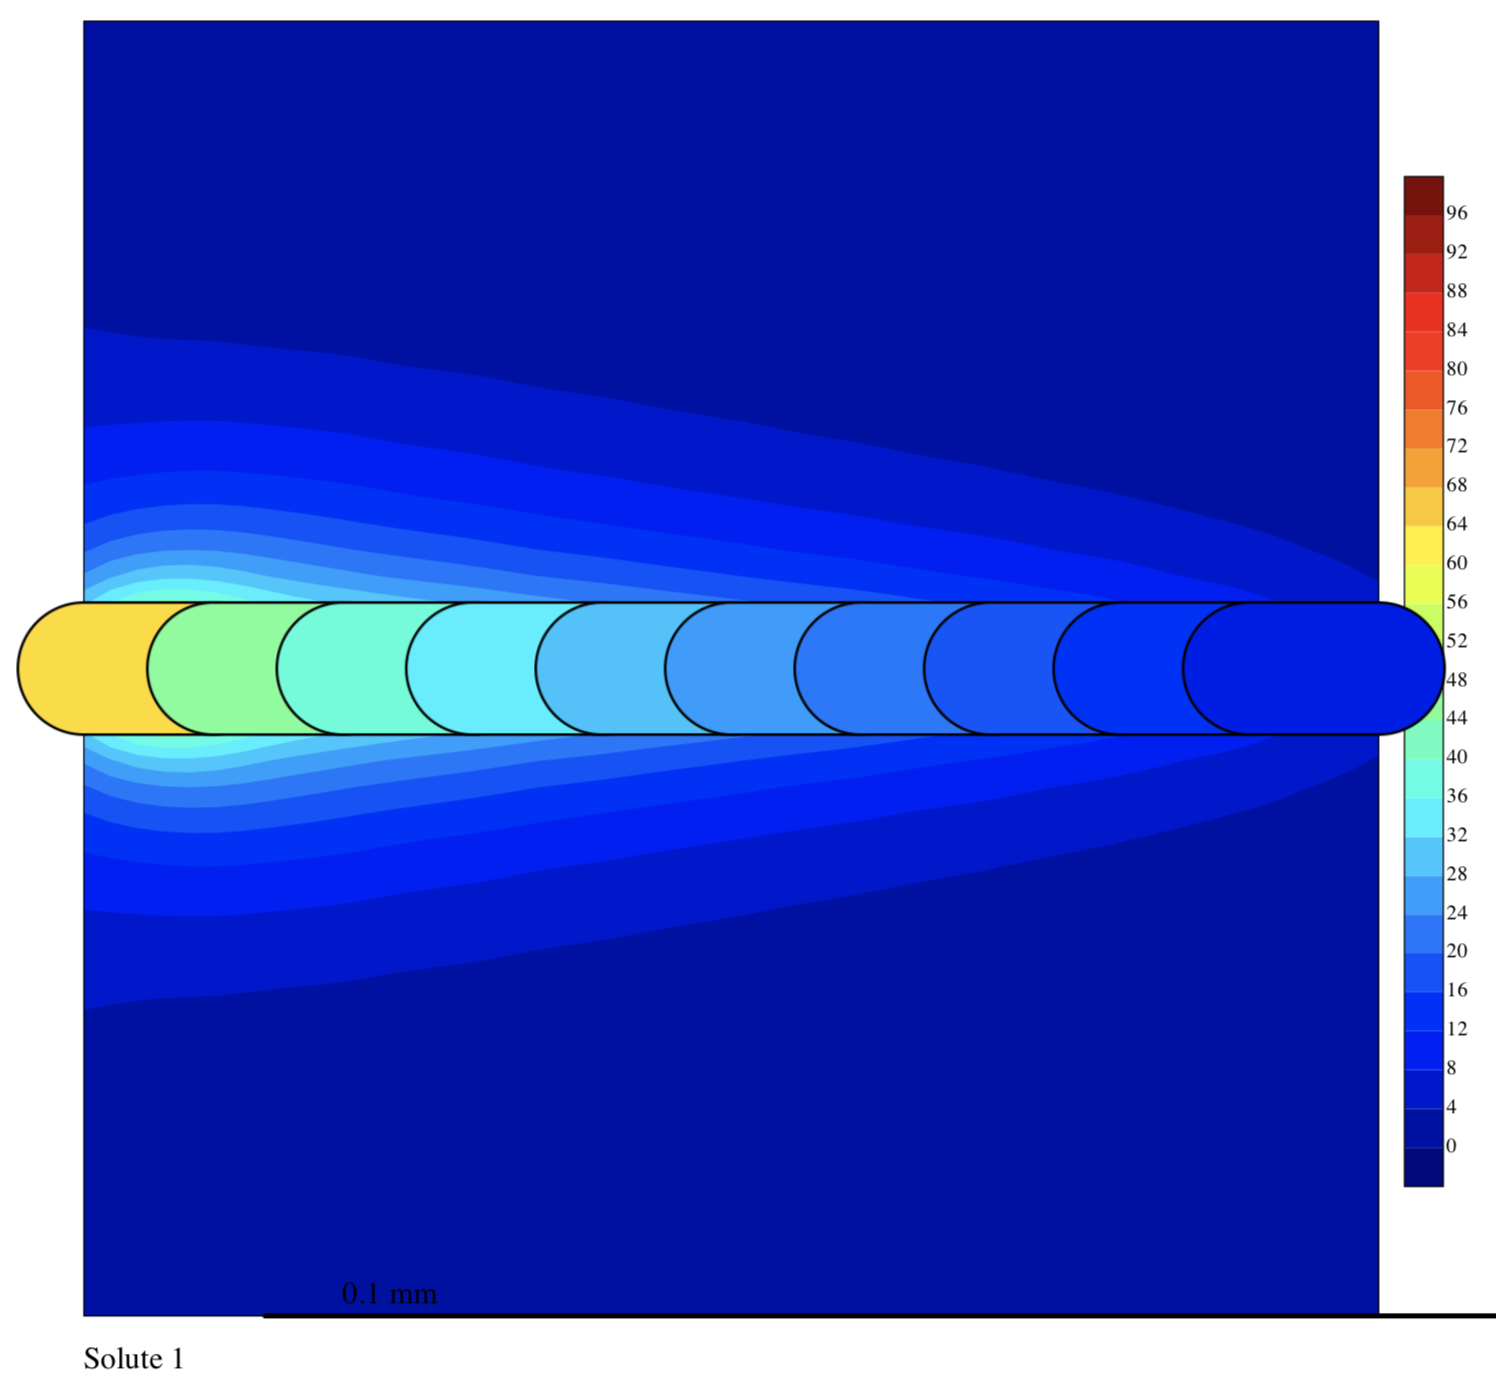
\includegraphics[width=120mm]{Contour_Krogh}
\caption{\footnotesize Green's Contour Output for Krogh Network}
\label{fig:Contour_Krogh}
\end{figure}

%\subsubsection*{Brain Model}
%Explain relevance of this model and the produced results (many plots here)

%The Brain network provided by Secomb (?) was used for further simulations and to validate the produced data.

\subsubsection*{Cardiac Model}
%Explain relevance of this model and the produced results (many plots here)

The Cardiac network provided by Secomb (?) was used for further simulations and to validate the produced data.\\
\\Figure \ref{fig:Contour_Cardiac1}  is the result of a Green's Method blood flow simulation computed on a Cardiac network. The Solute Concentration in the network is visualized.\\
\begin{figure}[h]
\centering
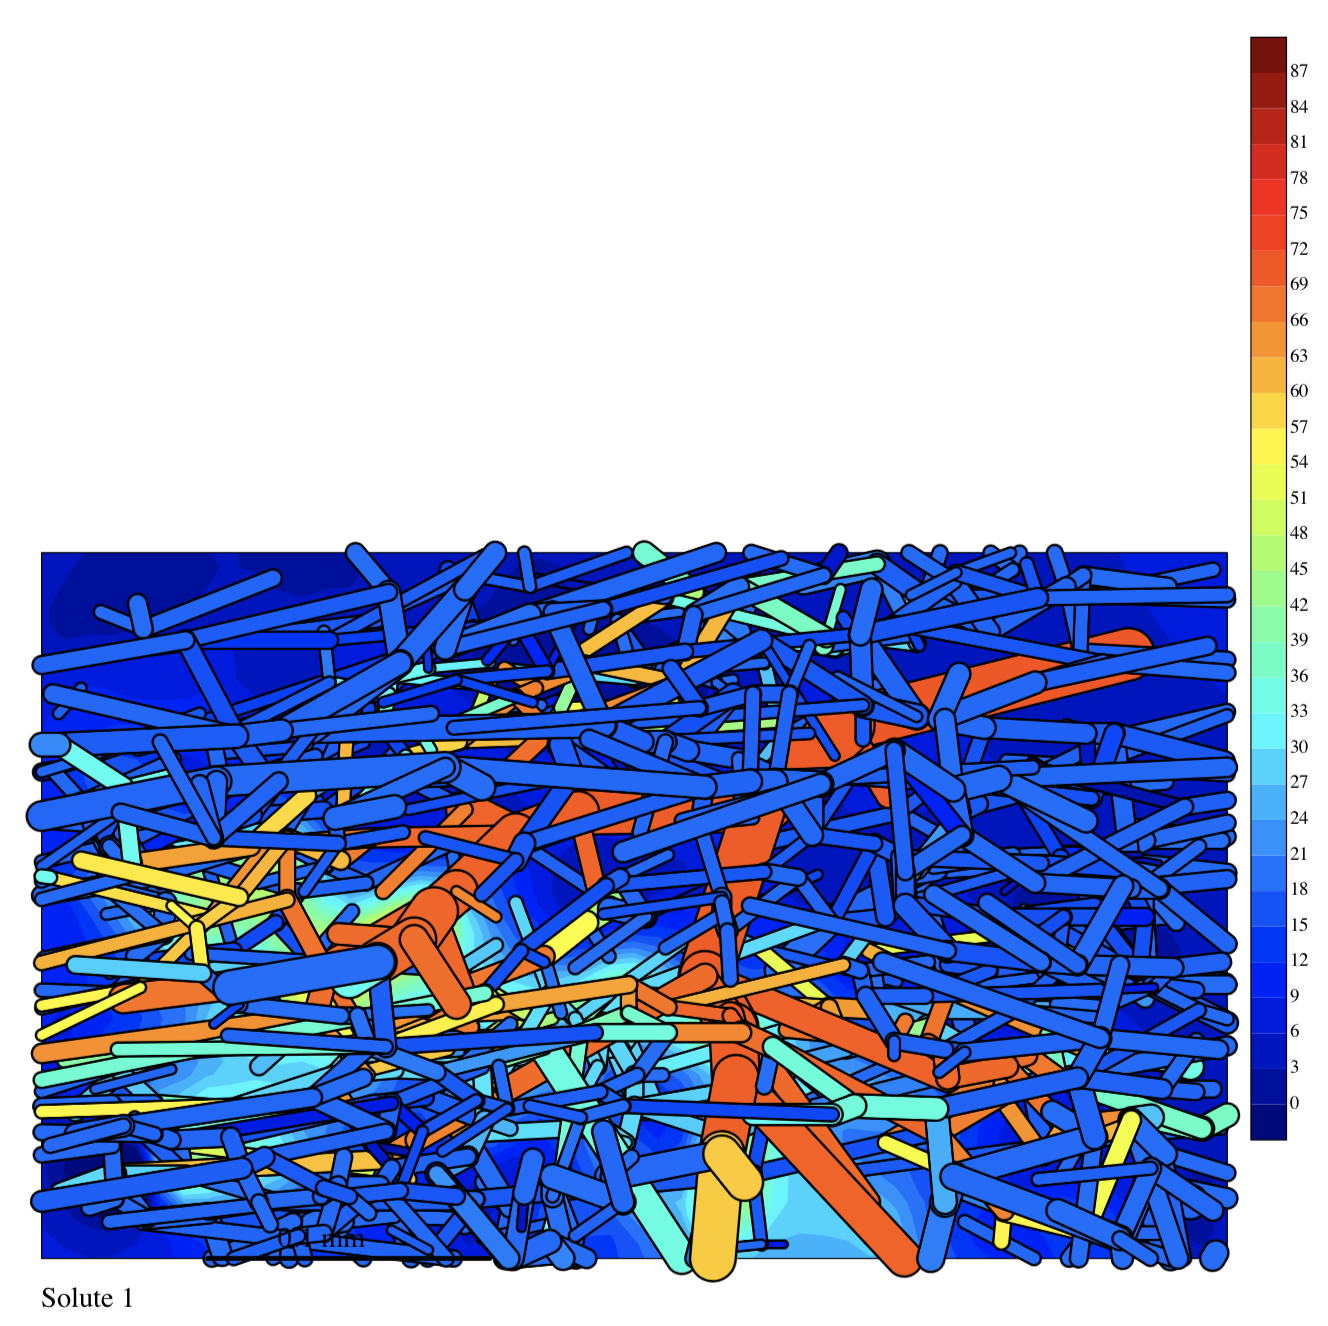
\includegraphics[width=85mm]{Contour_Cardiac}
\caption{\footnotesize Green's Contour Output for Cardiac Network}
\label{fig:Contour_Cardiac1}
\end{figure}

\subsubsection*{Mescent Model}
%Explain relevance of this model and the produced results (many plots here)

The Mescent network provided by Secomb (?) was used for further simulations and to validate the produced data.\\
\\Figure \ref{fig:Contour_Mescent1}  is the result of a Green's Method blood flow simulation computed on a Mescent network. The Solute Concentration of Solute 1 in the network is visualized.\\
\begin{figure}[h]
\centering
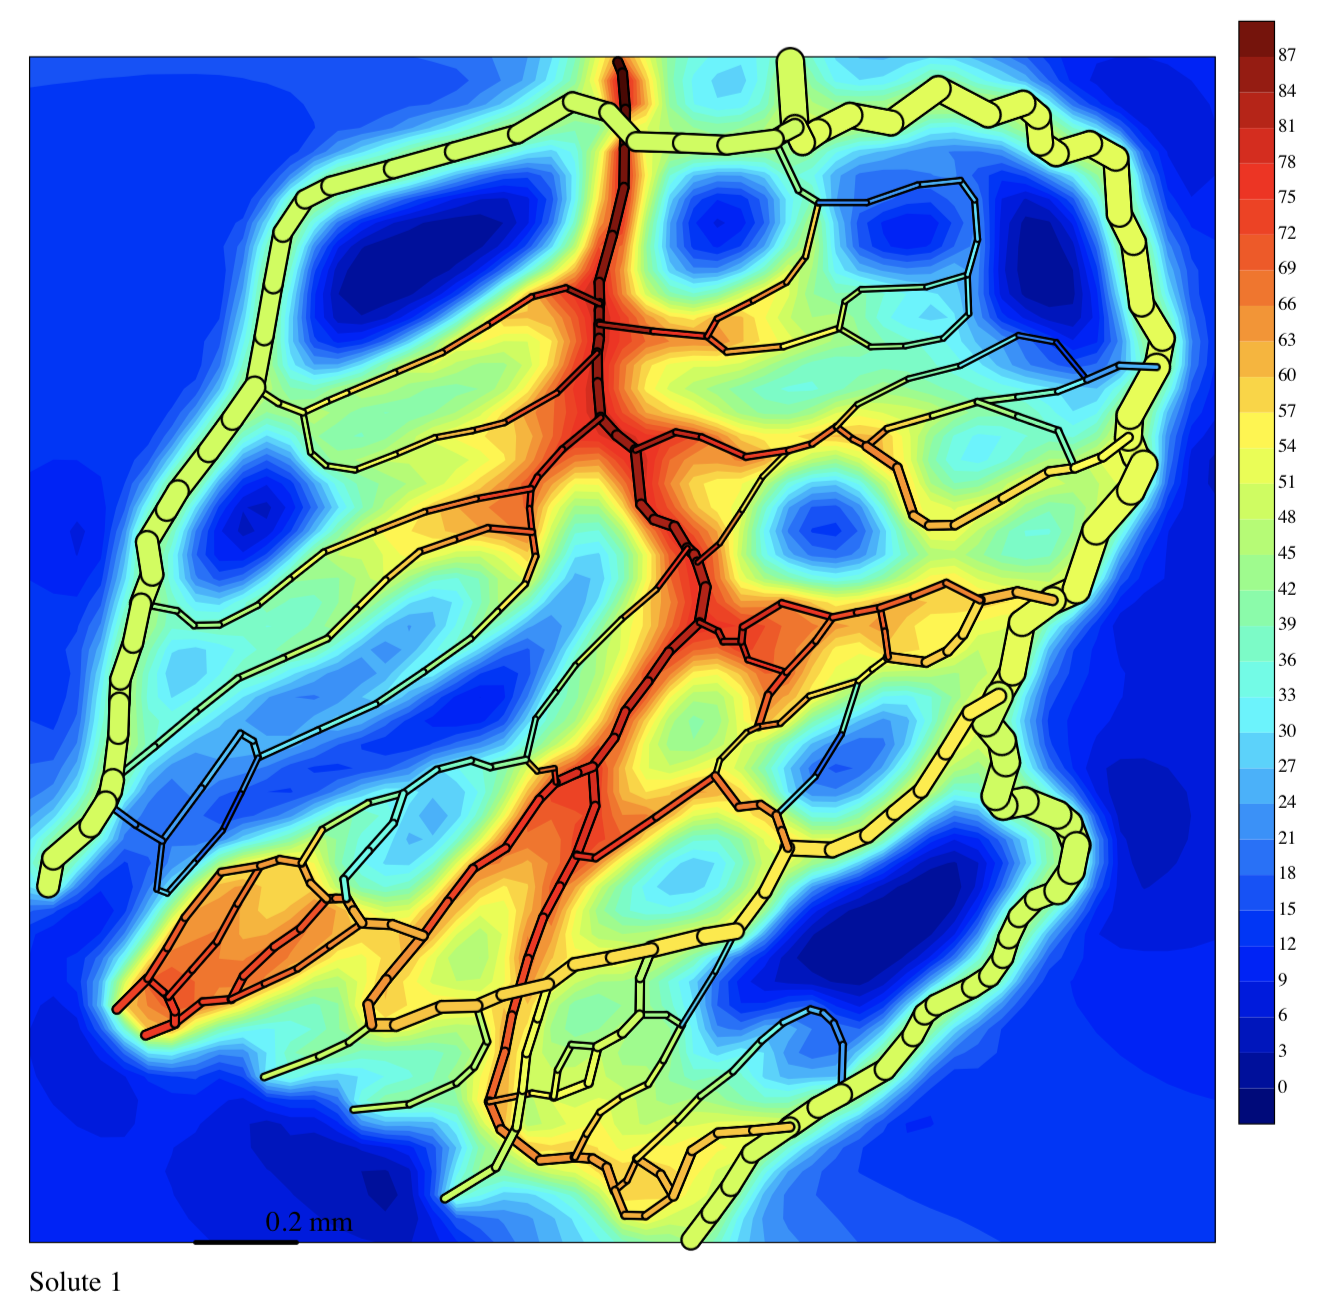
\includegraphics[width=85mm]{Contour_Mescent1}
\caption{\footnotesize Green's Contour Output for Mescent Network (Solute 1)}
\label{fig:Contour_Mescent1}
\end{figure}\\
%
\\Figure \ref{fig:Contour_Mescent2}  is the result of a Green's Method blood flow simulation computed on a Mescent network. The Solute Concentration of Solute 2 in the network is visualized.\\
\begin{figure}[h]
\centering
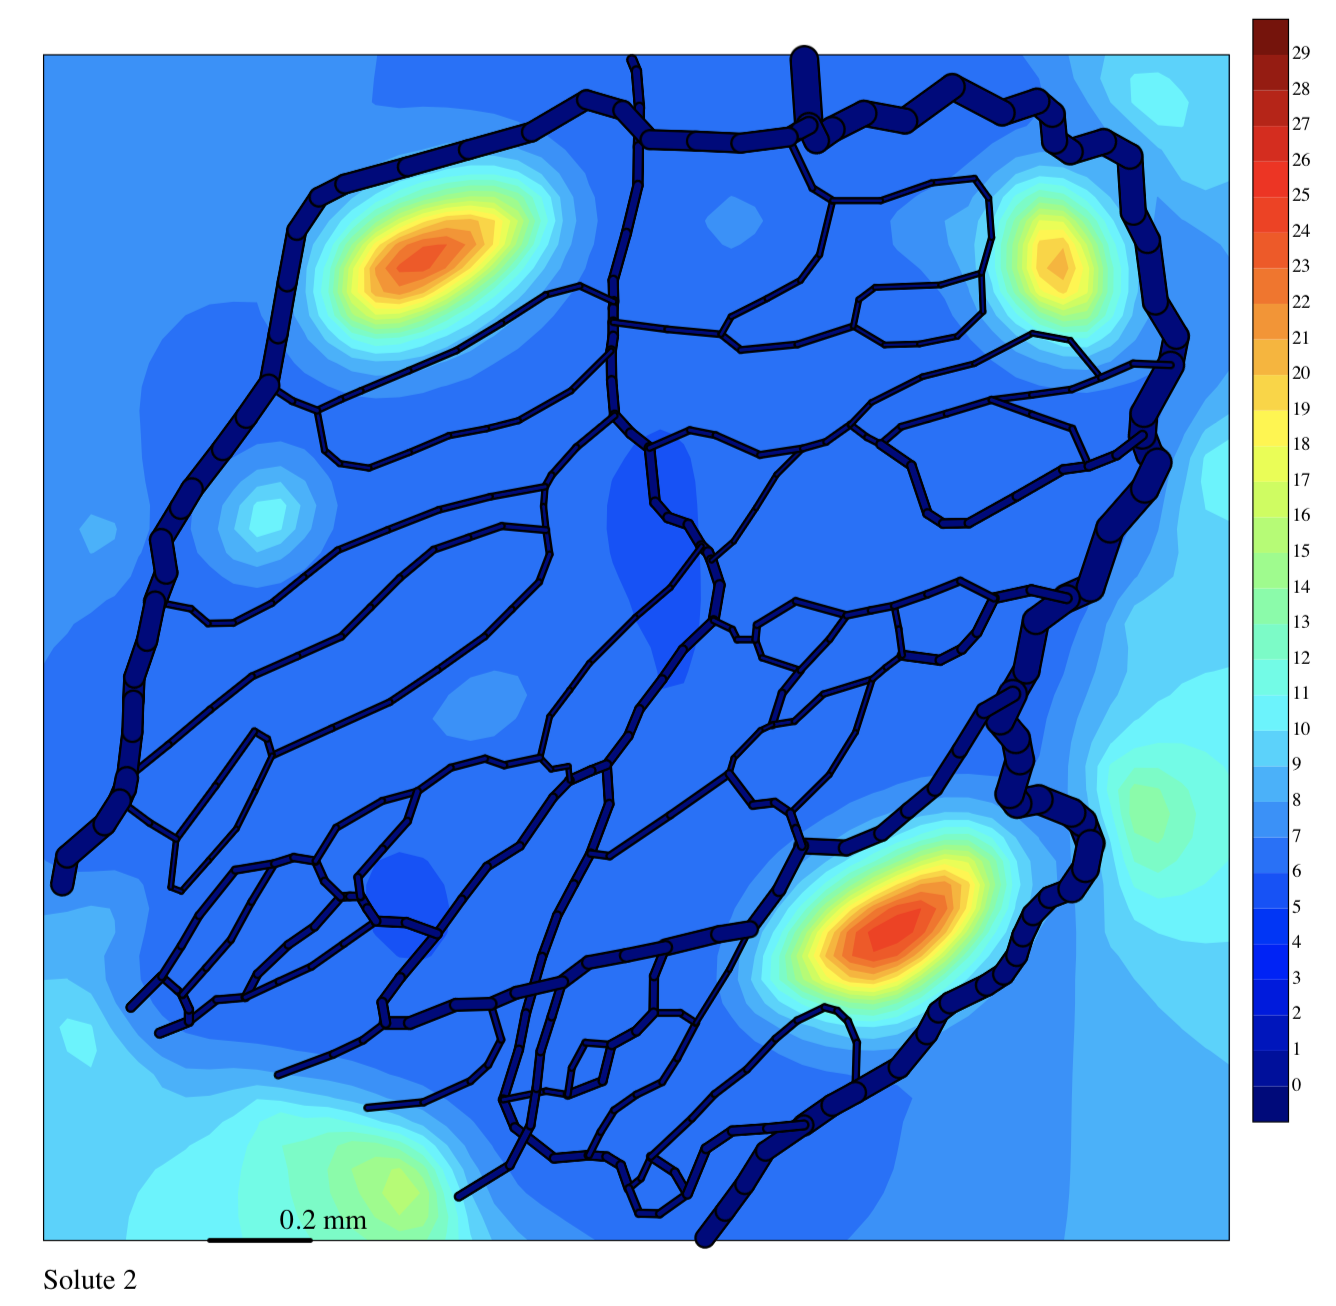
\includegraphics[width=85mm]{Contour_Mescent2}
\caption{\footnotesize Green's Contour Output for Mescent Network (Solute 2)}
\label{fig:Contour_Mescent2}
\end{figure}

\subsubsection*{Tumor Model}
%Explain relevance of this model and the produced results (many plots here)

The Tumor network provided by Secomb (?) was used for further simulations and to validate the produced data.
Figure \ref{fig:Contour_Cardiac1}  is the result of a Green's Method blood flow simulation computed on a Tumor network. The Solute Concentration in the network is visualized.\\
\begin{figure}[h]
\centering
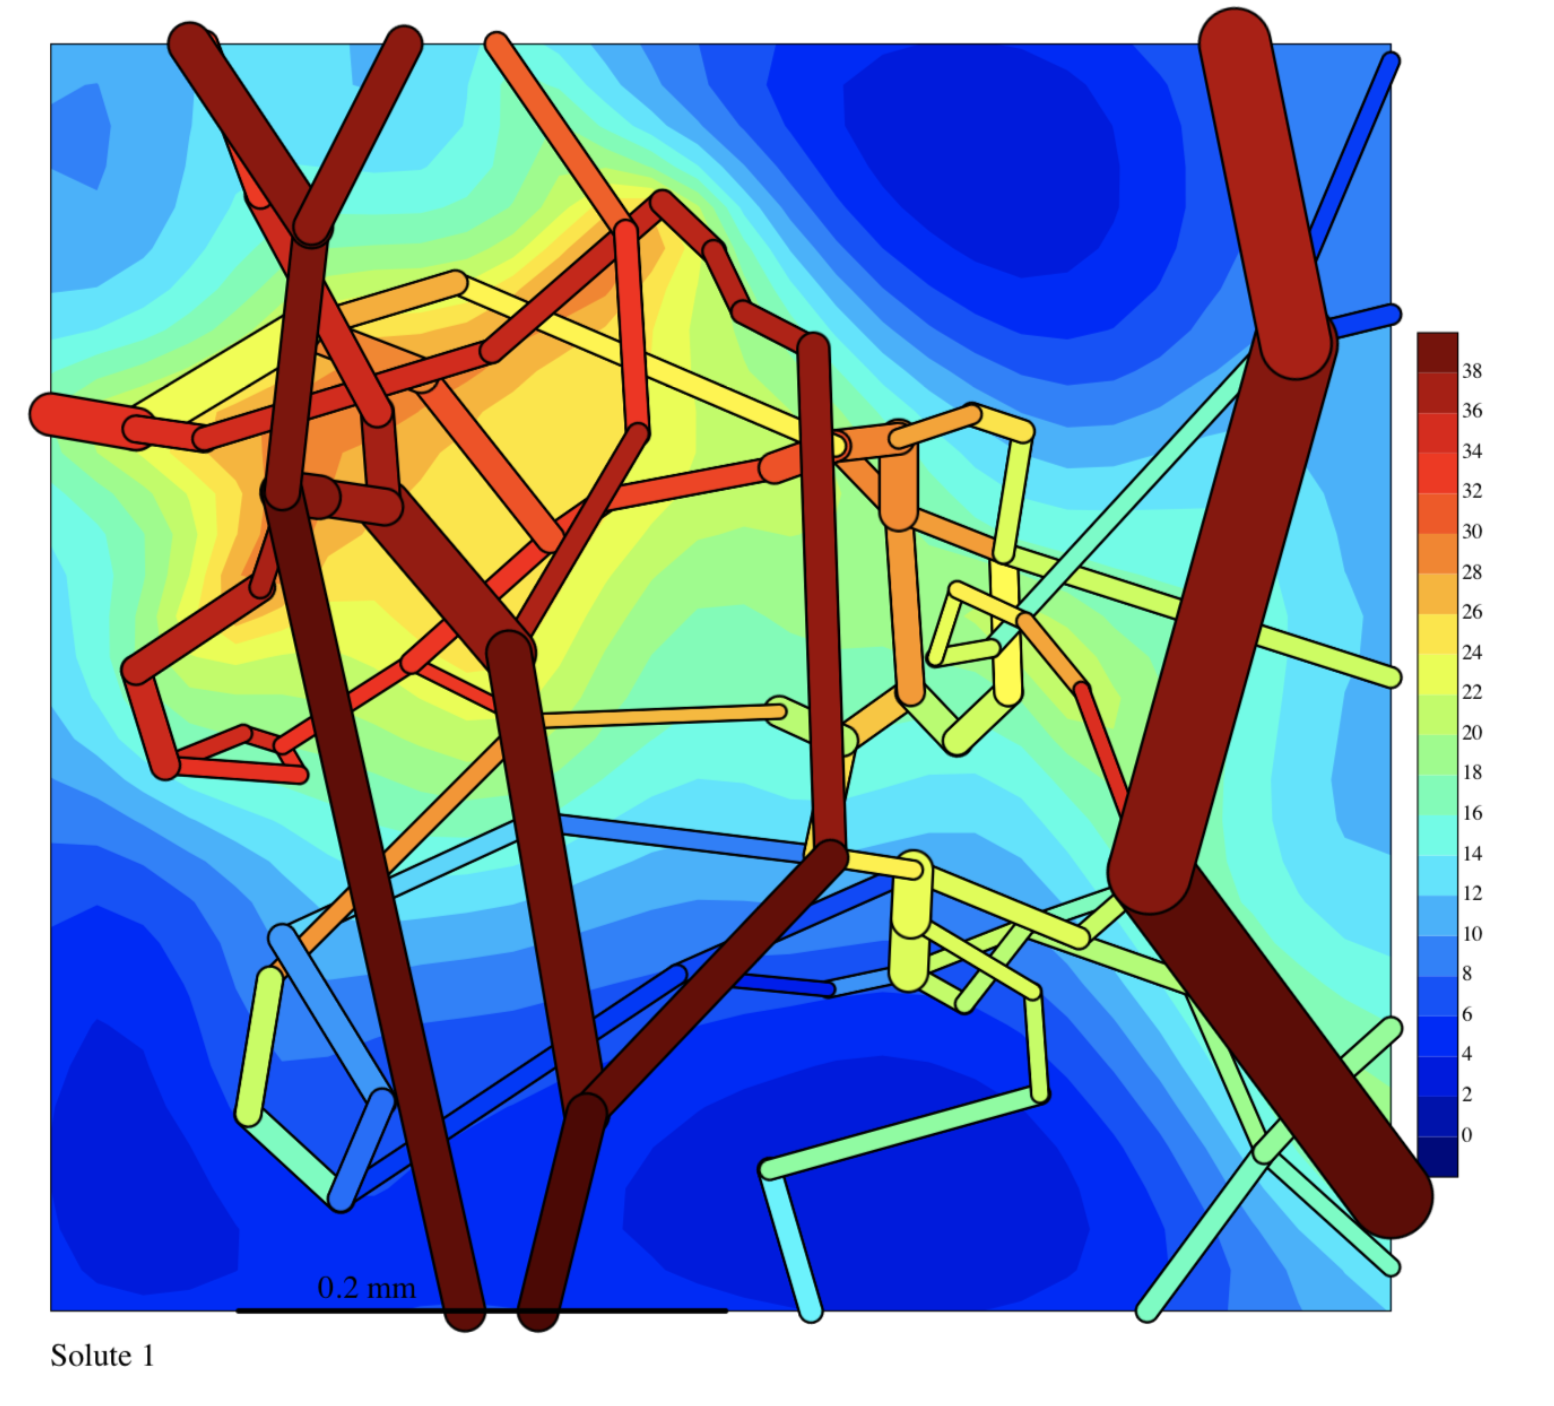
\includegraphics[width=75mm]{Contour_Tumor}
\caption{\footnotesize Green's Contour Output for Tumor Network}
\label{fig:Contour_Tumor}
\end{figure}

\subsubsection*{Further Outlook for New Networks}
%Explain relevance of the new models and the produced results (many plots here)

The results provided by the Green's Method Code were previously discussed for a few networks provided by Secomb (?). In this section the goal is to see how this method can perform in general when it is applied to new networks and to discuss the produced results in detail.

\subsubsection{Discussion of Green's Method and the Produced Results}
%Discussion part of Green's

Final thoughts about Green's Method for physiological applications and oxygen delivery simulations/computations.

\subsection{$DuMu^x$}
%Explain DuMuX in general and explain the implemented method.

$DuMu^x$ is an open source software developed by a strong user community everywhere in the world. The software was basically developed by the University of Stuttgart, and provides a C++ based library of numerical methods and implemented test models, to simulate and solve transport and flow processes in porous media as described in \cite{flemisch2007dumux}.

\subsubsection{General Structure of $DuMu^x$}
%Explain how DuMuX works and what is interesting about it.

$DuMu^x$ is a multi-scale multi-physics toolbox that aims to describe the physical properties of a specific problem as correct as possible, by focussing on minimizing the computational cost \cite{flemisch2007dumux}.\\
\\The structure of $DuMu^x$ is specified in this chapter and illustrated with some figures.
Figure \ref{fig:dumux_structure}  is the Structure of $DuMu^x$ given from the $DuMu^x$ Version 2.12 Documentation \cite{flemischdumux}.\\
\begin{figure}[p]
\centering
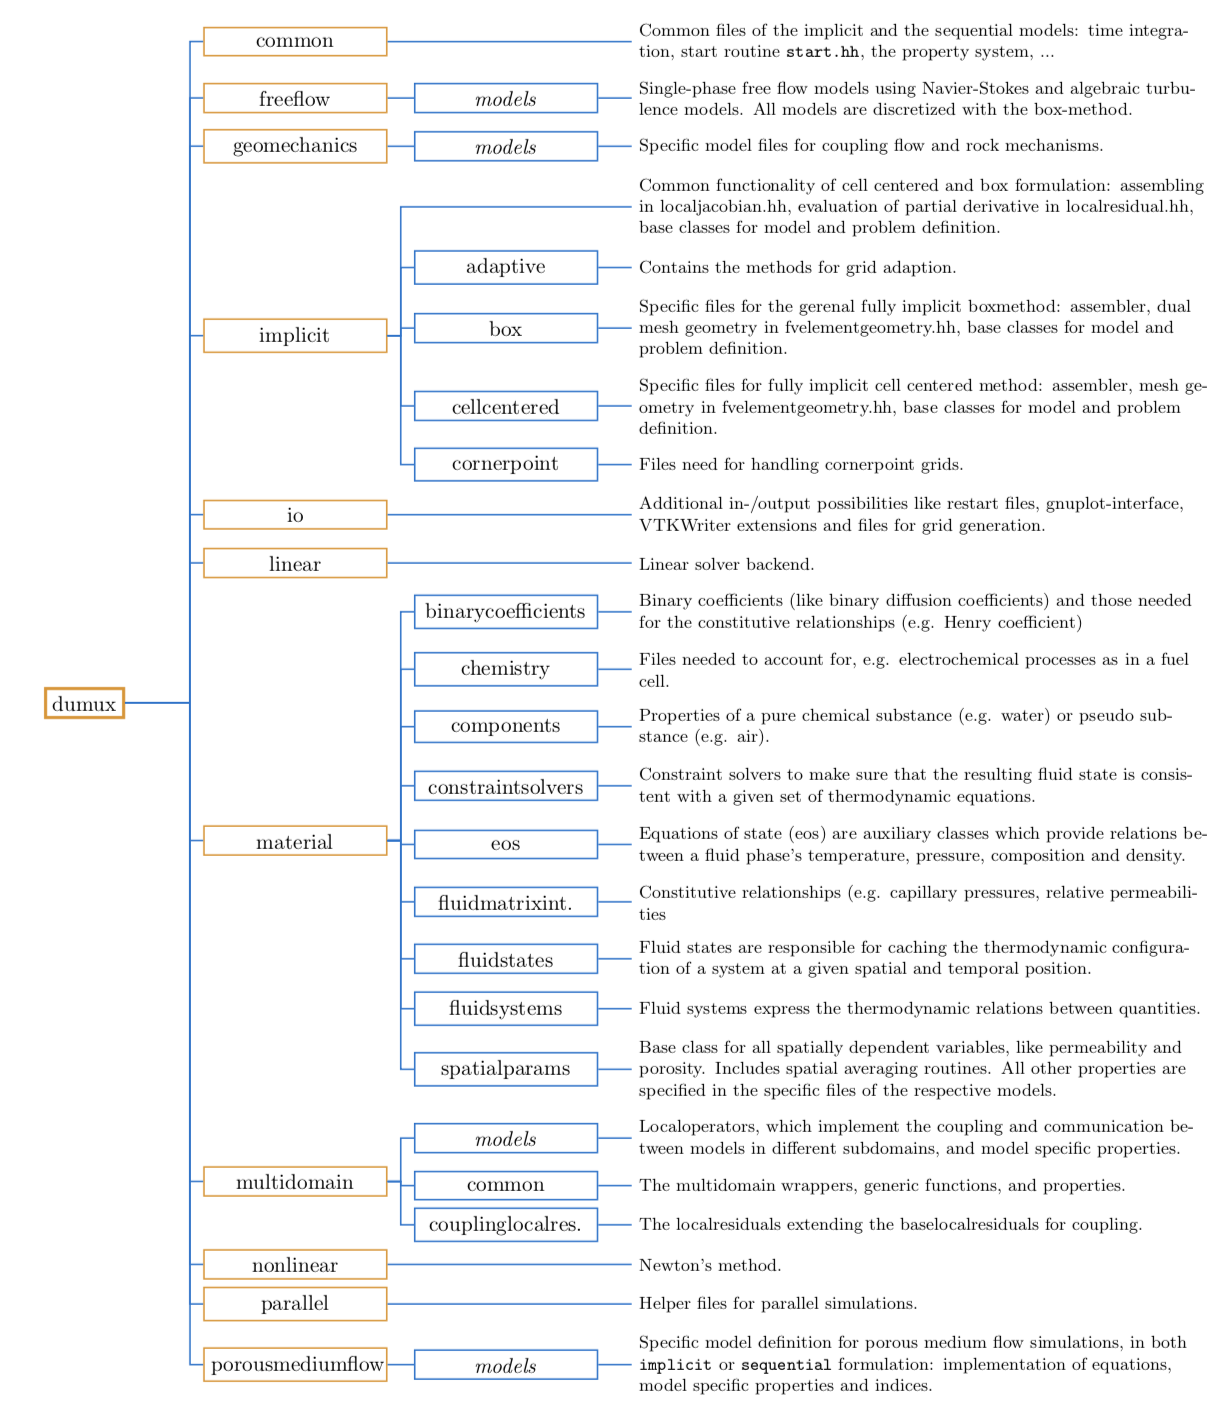
\includegraphics[height=190mm]{dumux_structure}
\caption{\footnotesize The $DuMu^x$ Structure}
\label{fig:dumux_structure}
\end{figure}\\\\\\\\\\\\\\\\\\\\

\subsubsection{Implemented Model}
%Explain Coupling of Tracer.

While $DuMu^x$ has a modular structure, some of the existing test cases can be combined to solve a more sophisticated and specific problem. In our case, this refers to the coupling of the existing Tracer model to the 1p-1p model. While the 1p-1p model can simulate the flow of a solute in a network by convection and the diffusion of this solute into tissue, the tracer model can literally trace the path of this solute into the tissue, which can be used to obtain Oxygen transport and diffusion into the tissue.

\subsubsection{Input Data for the Simulations}
%Explain where the networks come from: CT by Willy and Artery/Vein recognition by Diego

The networks that were used for the simulations are extracted from real organs coming from mice. This process is done by scientists from different areas of expertise and is usually performed in the following order:
\\1)CT of the kidneys
\\2)Recognition of fat, tissue, arteries and veins by machine learning algorithms
\\3)Three dimensional captions of the organ are build by many virtual two dimensional slices
\\4)Transformation of the recognized artery/vein data into networks that can be used for the simulations.

\subsubsection{Results}
%Results part of DuMuX
-Pros/Cons
\\-Quality of results
\\-Paraview Visualization of results

\subsubsection*{Some Nord Network Simulations}

Figure \ref{fig:nord_pressure}  is the result of a $DuMu^x$ blood flow simulation computed on a Nord network. The pressure field in the network is visualized.\\
\begin{figure}[h]
\centering
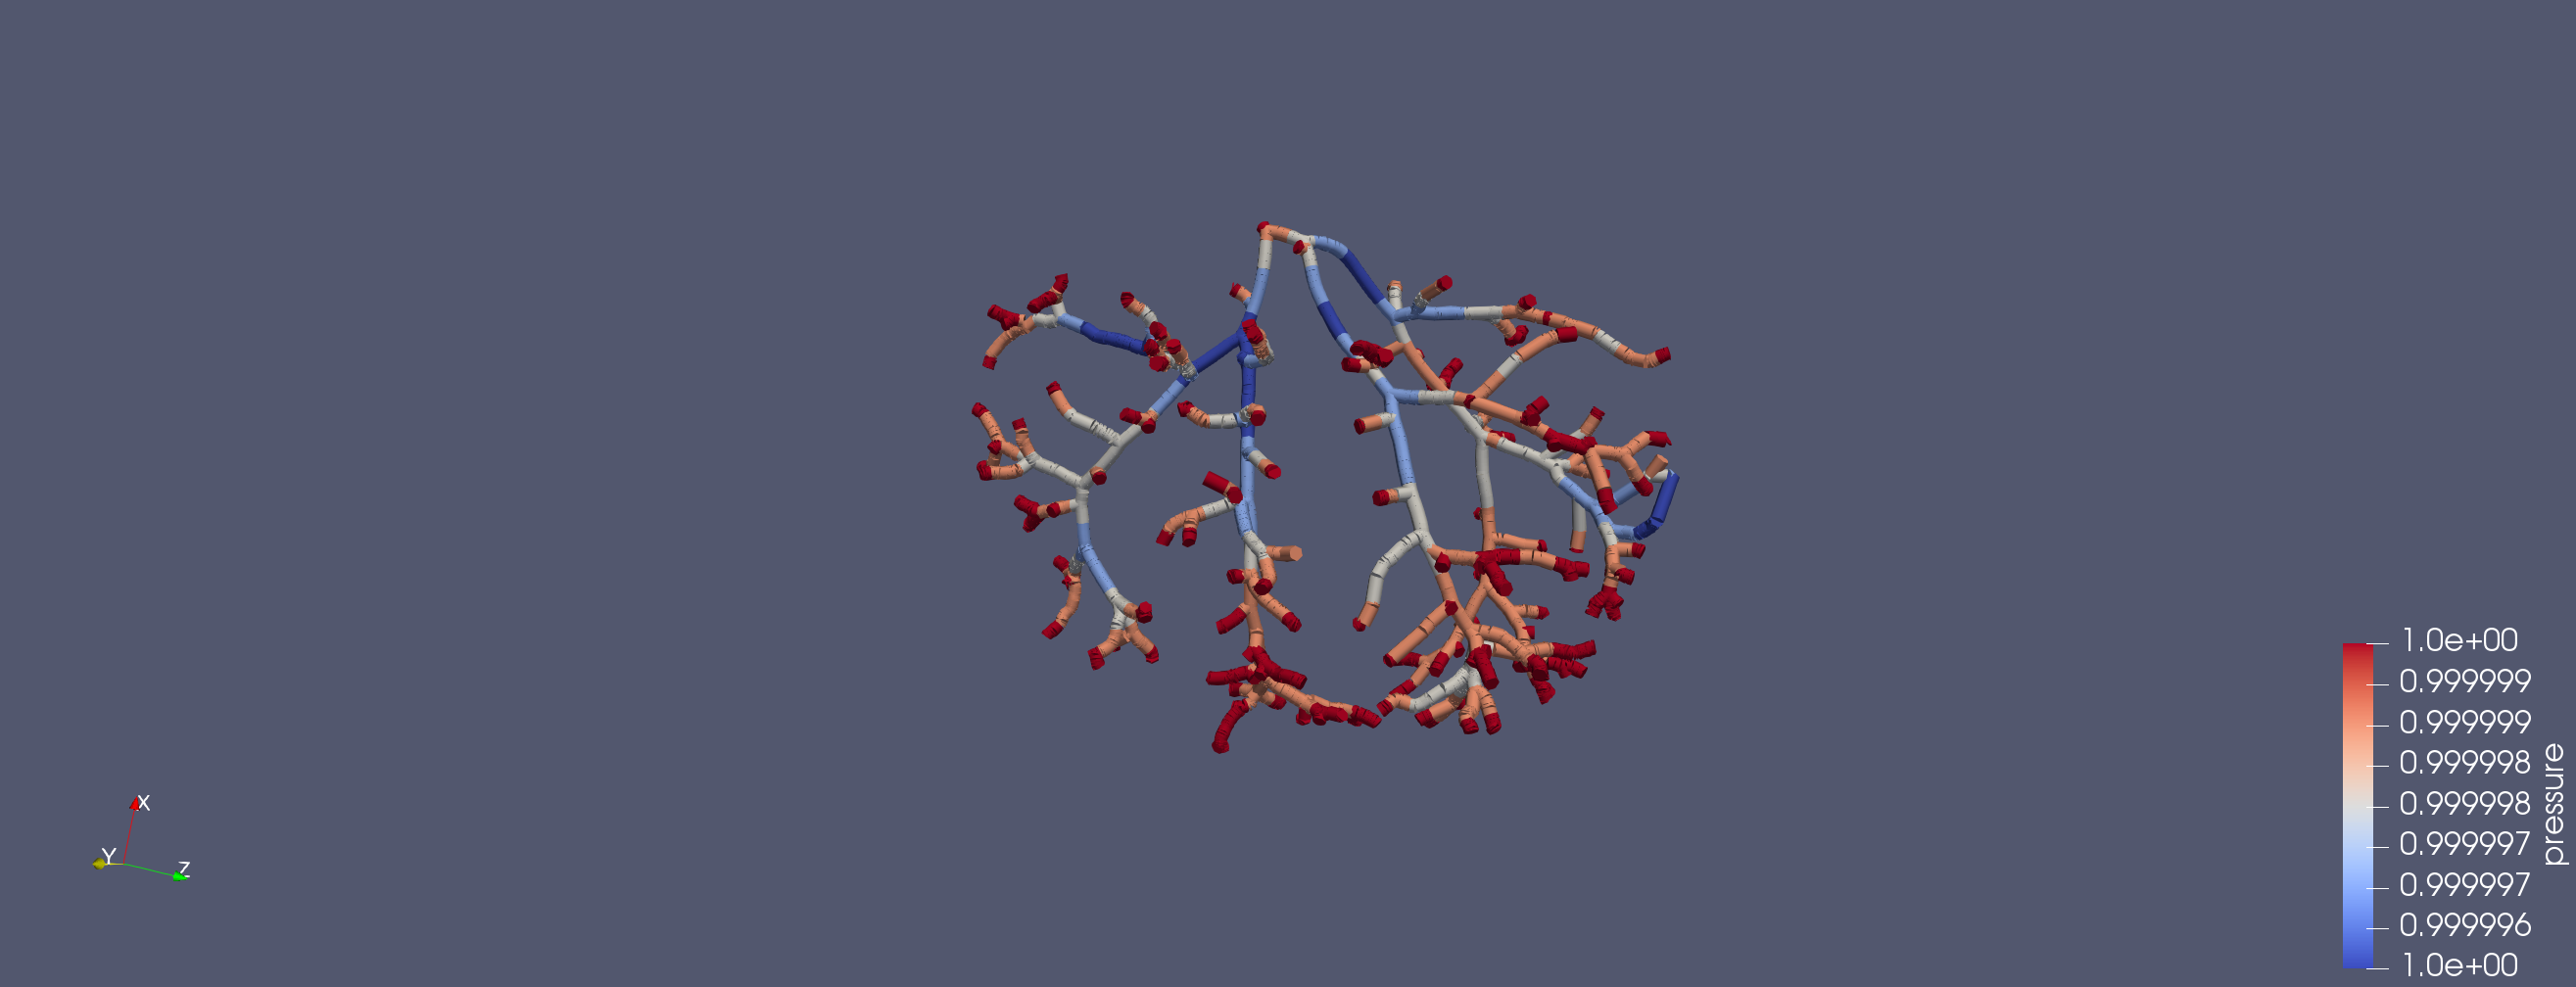
\includegraphics[width=180mm]{nord_pressure}
\caption{\footnotesize $DuMu^x$ Pressure Computations for Nord Network}
\label{fig:nord_pressure}
\end{figure}\\\\\\\\\\\\\\\\\\\\
%
\\Figure \ref{fig:nord_velocity}  is the result of a $DuMu^x$ blood flow simulation computed on a Nord network. The velocity field in the network is visualized.\\
\begin{figure}[h]
\centering
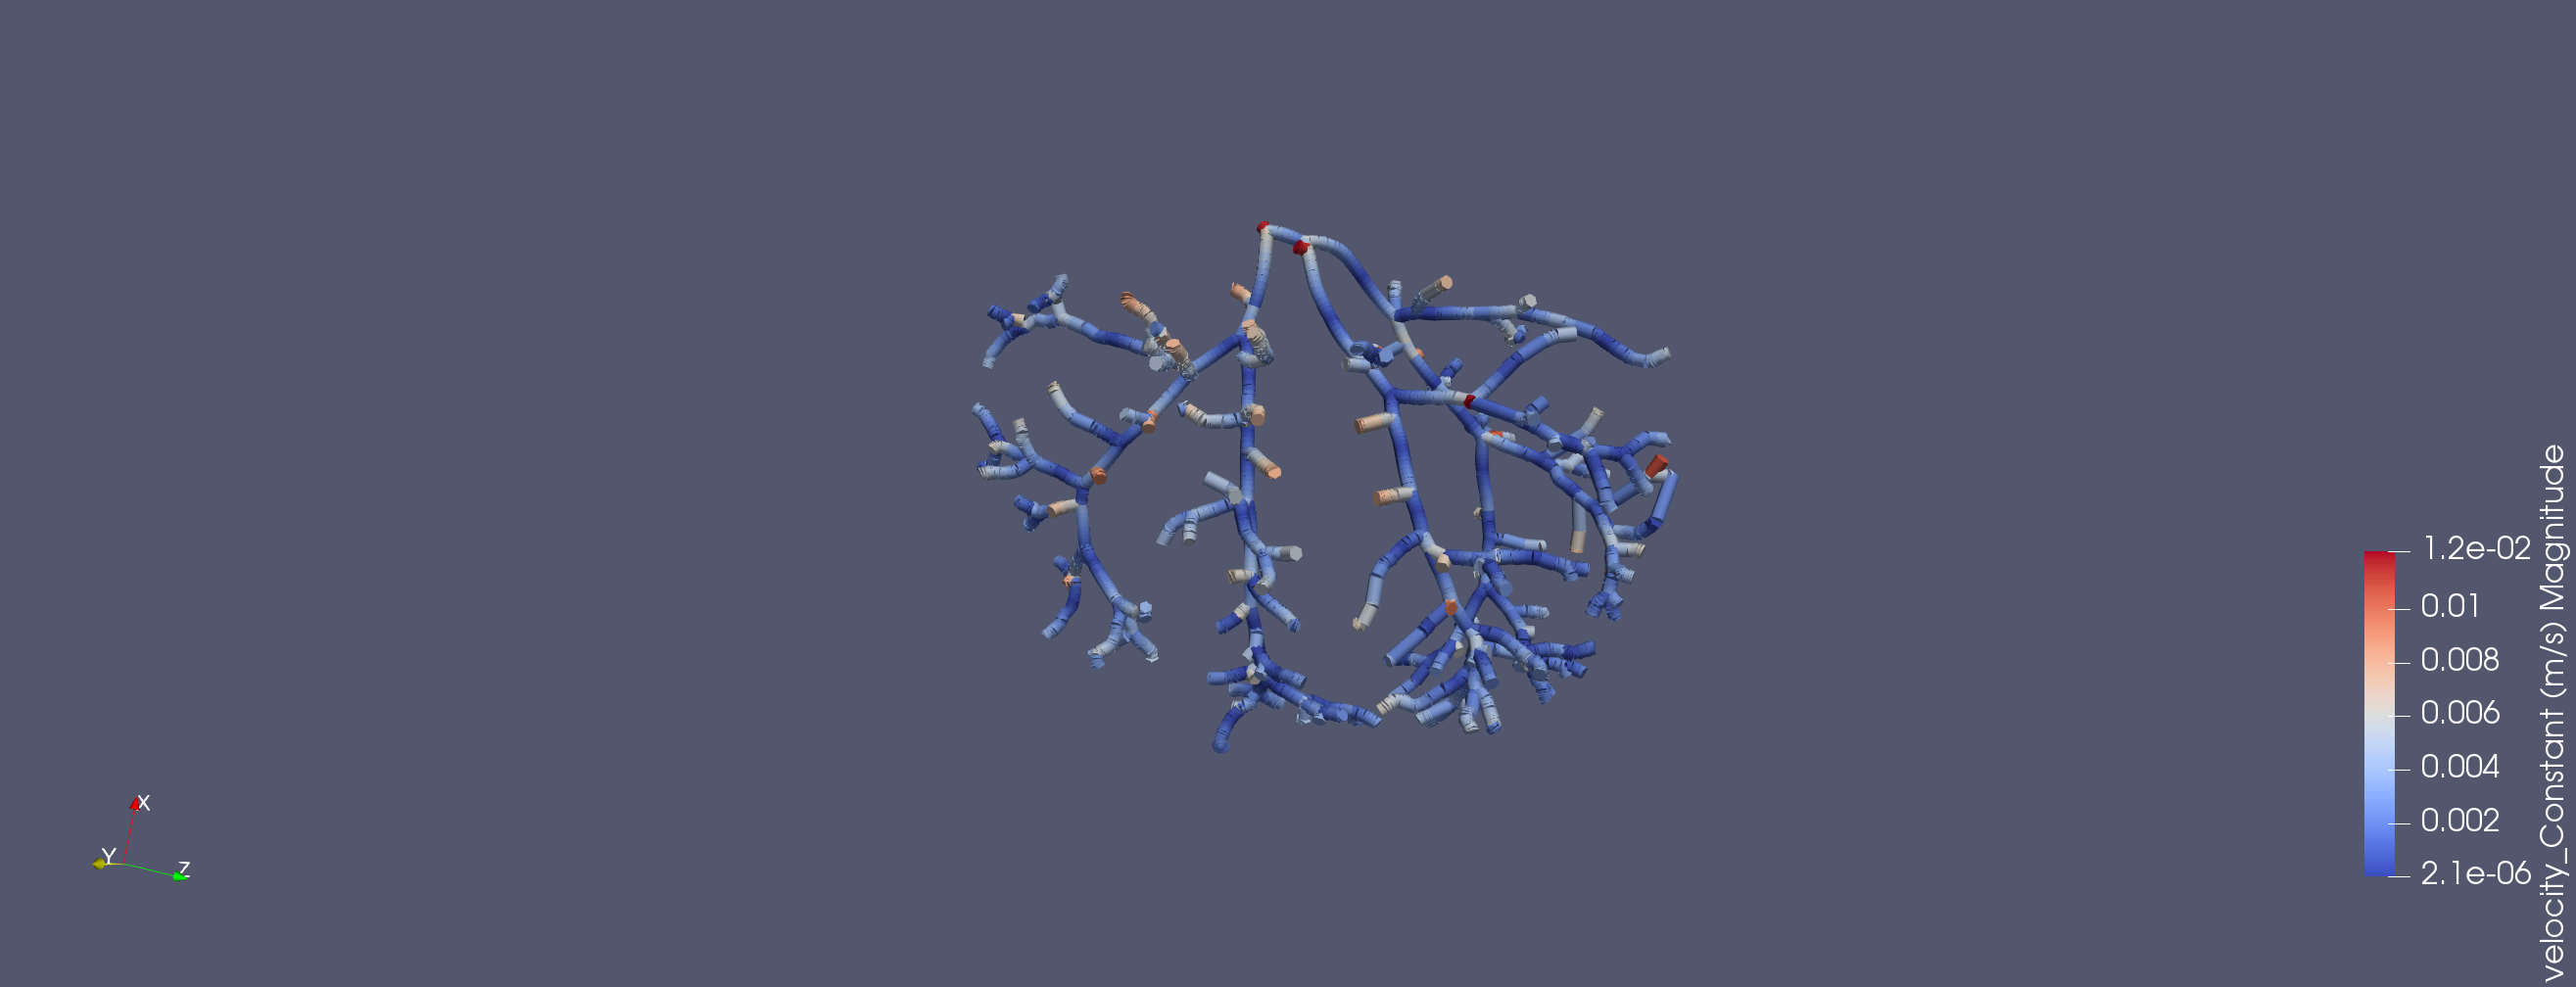
\includegraphics[width=180mm]{nord_velocity}
\caption{\footnotesize $DuMu^x$ Velocity Computations for Nord Network}
\label{fig:nord_velocity}
\end{figure}\\\\\\\\\\\\\\

\subsubsection*{Some Nephron Network Simulations}

Figure \ref{fig:nephron_pressure}  is the result of a $DuMu^x$ blood flow simulation computed on a Nephron network. The pressure field in the network is visualized.\\
\begin{figure}[h]
\centering
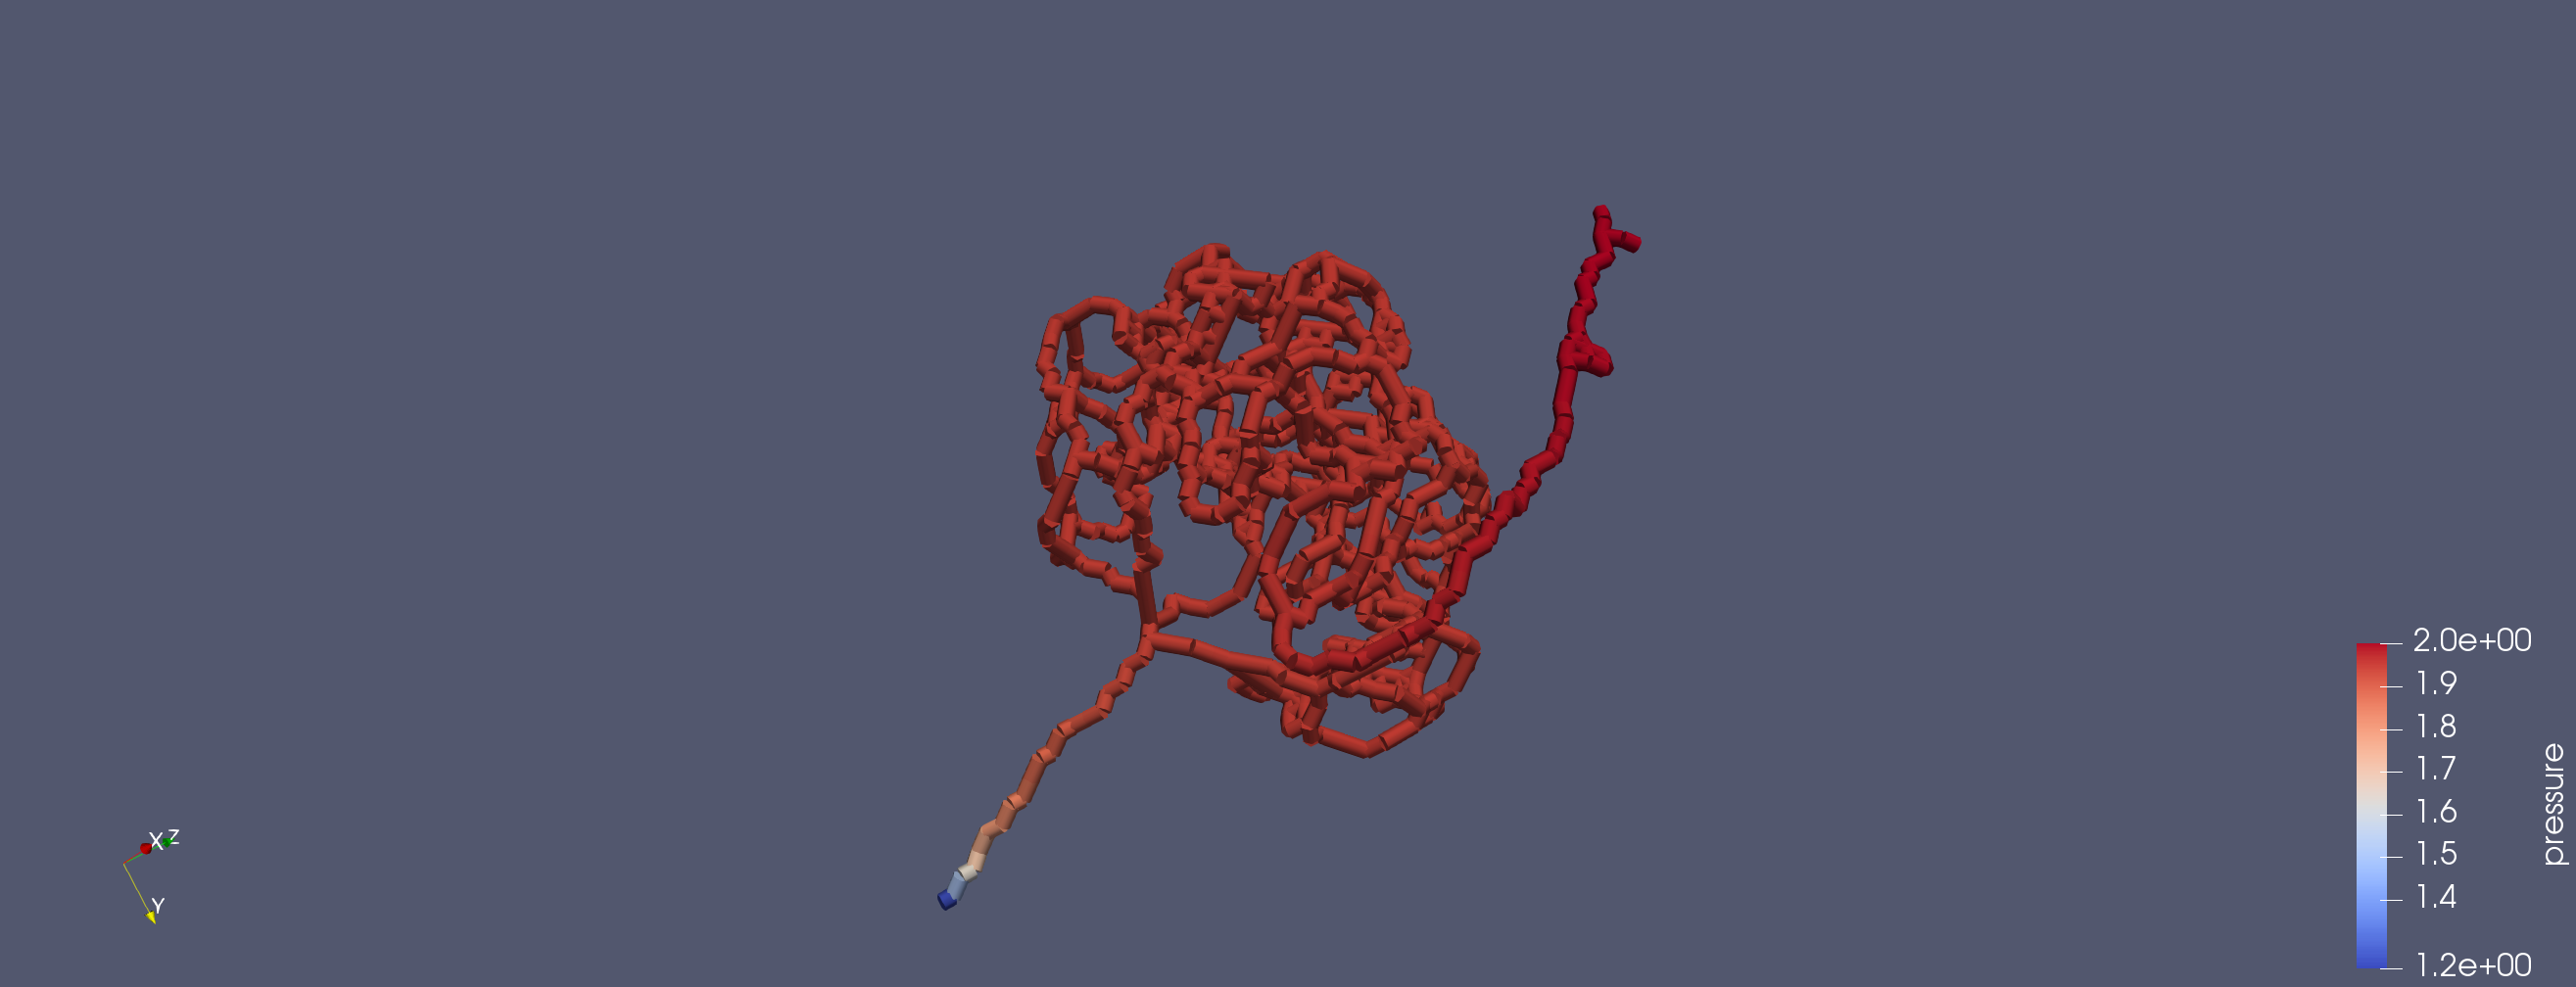
\includegraphics[width=180mm]{nephron_pressure}
\caption{\footnotesize $DuMu^x$ Pressure Computations for Nephron Network}
\label{fig:nephron_pressure}
\end{figure}\\
%
\\Figure \ref{fig:nephron_velocity}  is the result of a $DuMu^x$ blood flow simulation computed on a Nephron network. The velocity field in the network is visualized.\\
\begin{figure}[h]
\centering
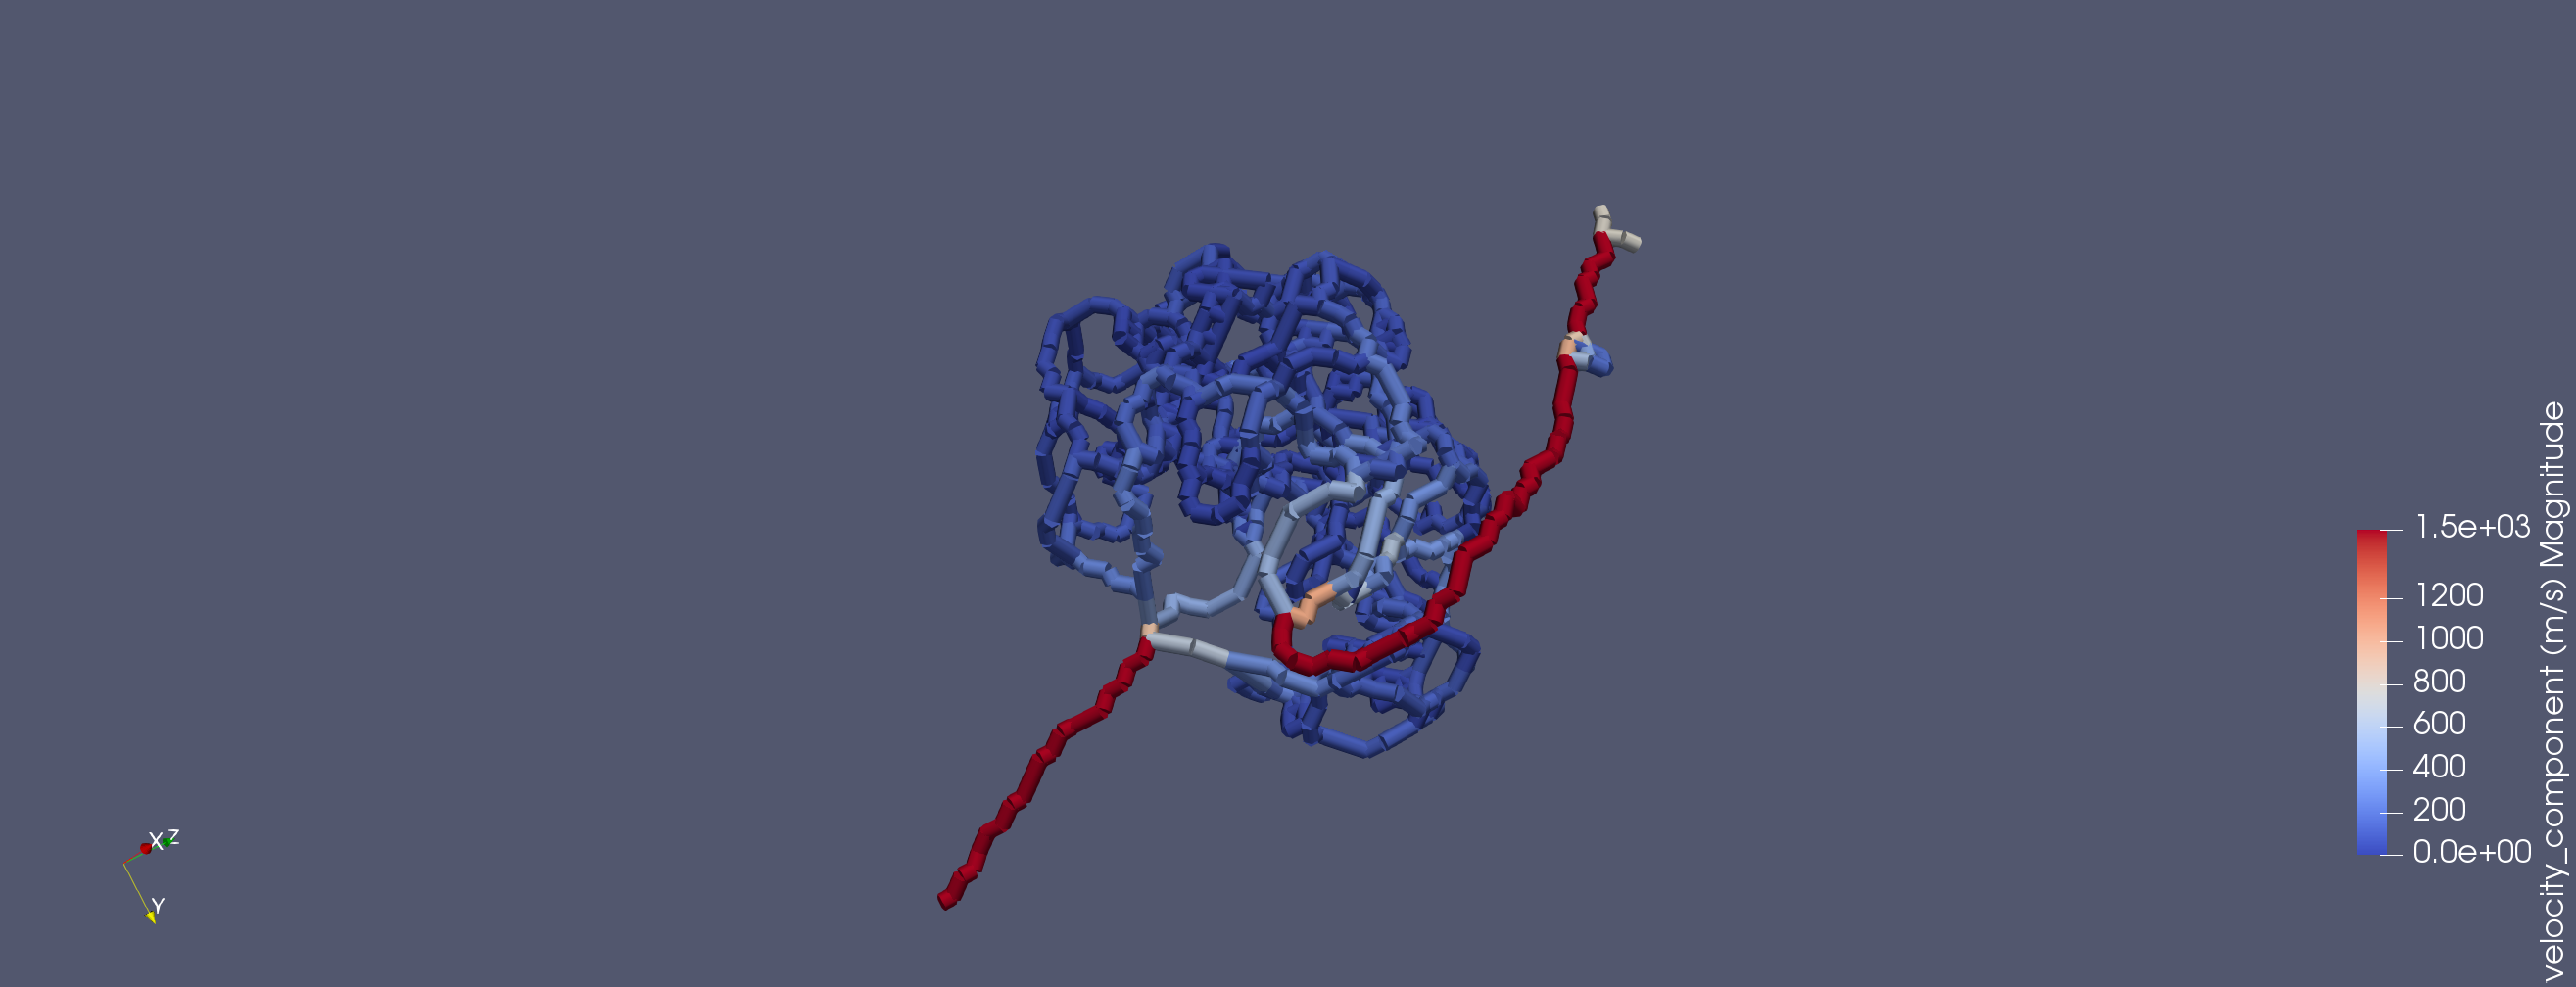
\includegraphics[width=180mm]{nephron_velocity}
\caption{\footnotesize $DuMu^x$ Velocity Computations for Nephron Network}
\label{fig:nephron_velocity}
\end{figure}\\\\

\section{Comparison of the Different Methods Behind the Simulations}
%Compare DuMuX to Green's Method in general
In this section the main differences between these two simulation methods described previously will be discussed.

\subsection{Comparison of the Results}
%Compare the produced results
In this section the main differences in the produced results for the same input files/same networks will be discussed.

\subsection{Comparison of the Numerical Methods}
%Compare the Solvers behind the Methods
%Very useful tu use Secomb Paper Numerical Methods section here
In this section the main differences between the solvers and the associated numerical methods will be discussed.
\\
\\As mentioned previously, one of the huge advantages of $DuMu^x$ is the flexibility it provides in terms of solvers, and thus in terms of the numerical methods used for the computations. This means that it is often possible to pick a solver which is stable for the specific problem and the chosen discretization.
\\
\\This is obviously different for the Green's Method code, as there is no option of choosing a different solver than the one provided in the code. As discussed previously, this code is specifically implemented to solve and compute Oxygen (or other Solute) concentrations in the blood and the surrounding tissue, and the implemented method strongly relies on the stability of the Green's Method and the numerical methods behind the solver.

\subsubsection{Explanation of the Methods}
%Explain the Methods and differences between methods
%Very useful tu use Secomb Paper Numerical Methods section here
In this section, the focus will be the numerical methods behind the Green's Method code and $DuMu^x$ and the differences in their implementation.

\subsubsection{Stability Questions and Computational Cost}
%Explain when and why which the numerical methods are stable
In this section, the consequences of the previously described differences will be discussed. The focus lies on the differences in terms of stability and computational cost for similar simulations.


%\section{Discussion}

%I already did this previously, so might delete this part ...

\section{Conclusion}
%Summary of both methods in general and Outlook for the research field
%What this review was about: short summary. Main points
%highlighted. Perhaps a graph regrouping together elements.
%Comparison of different strategies and their state. Maybe your own
%thoughts on the whole story and where the promising directions lie
%and which ones you see with scepticism.

As seen previously, both the Green's Function Method and the implemented $DuMu^x$-based method can offer very interesting options. While the Green's Function Method is presenting a specifically created C++ based software for Oxygen Transport and Diffusion simulations, the results show that the obtained outputs are not always satisfying (eventually will happen for new networks?). The reasons for this have been discussed previously (maybe repeat them shortly here).
Compared to this, the $DuMu^x$ based model is still in its very initial phase and cannot produce correct results yet (very probably). Still, the fact that it is $DuMu^x$ based offers both a large flexibility to the user in terms of further development, as well as in terms of computational flexibility when choosing a time- and space-discretization through choosing discretization modules and different grid creators. The solvers can also be chosen by the user, which doesn't guarantee an overall stable numerical solver, but can provide great flexibility when adapting the model to specific networks.
\\
\\Main conclusions and final remarks.


\section{Acknowledgements}
Thank you all for the support blabla...

%\section{Conclusion}
Main conclusions and final remarks.


% Bibliography
\newpage
\addtocontents{toc}{\vspace{.5\baselineskip}}
\addcontentsline{toc}{section}{\protect\numberline{}{References}}
\bibliography{article}


% Appendices (if needed)
\addtocontents{toc}{\vspace{.5\baselineskip}}
\appendix
%!TEX root = article.tex

\section{Appendix}
\label{s:Appendix}

Additional material such as extra figures.
\subsection{DuMuX Results Visualized with ParaView}
%Put all the extra images from ParaView here.
\begin{figure}[h]
\centering
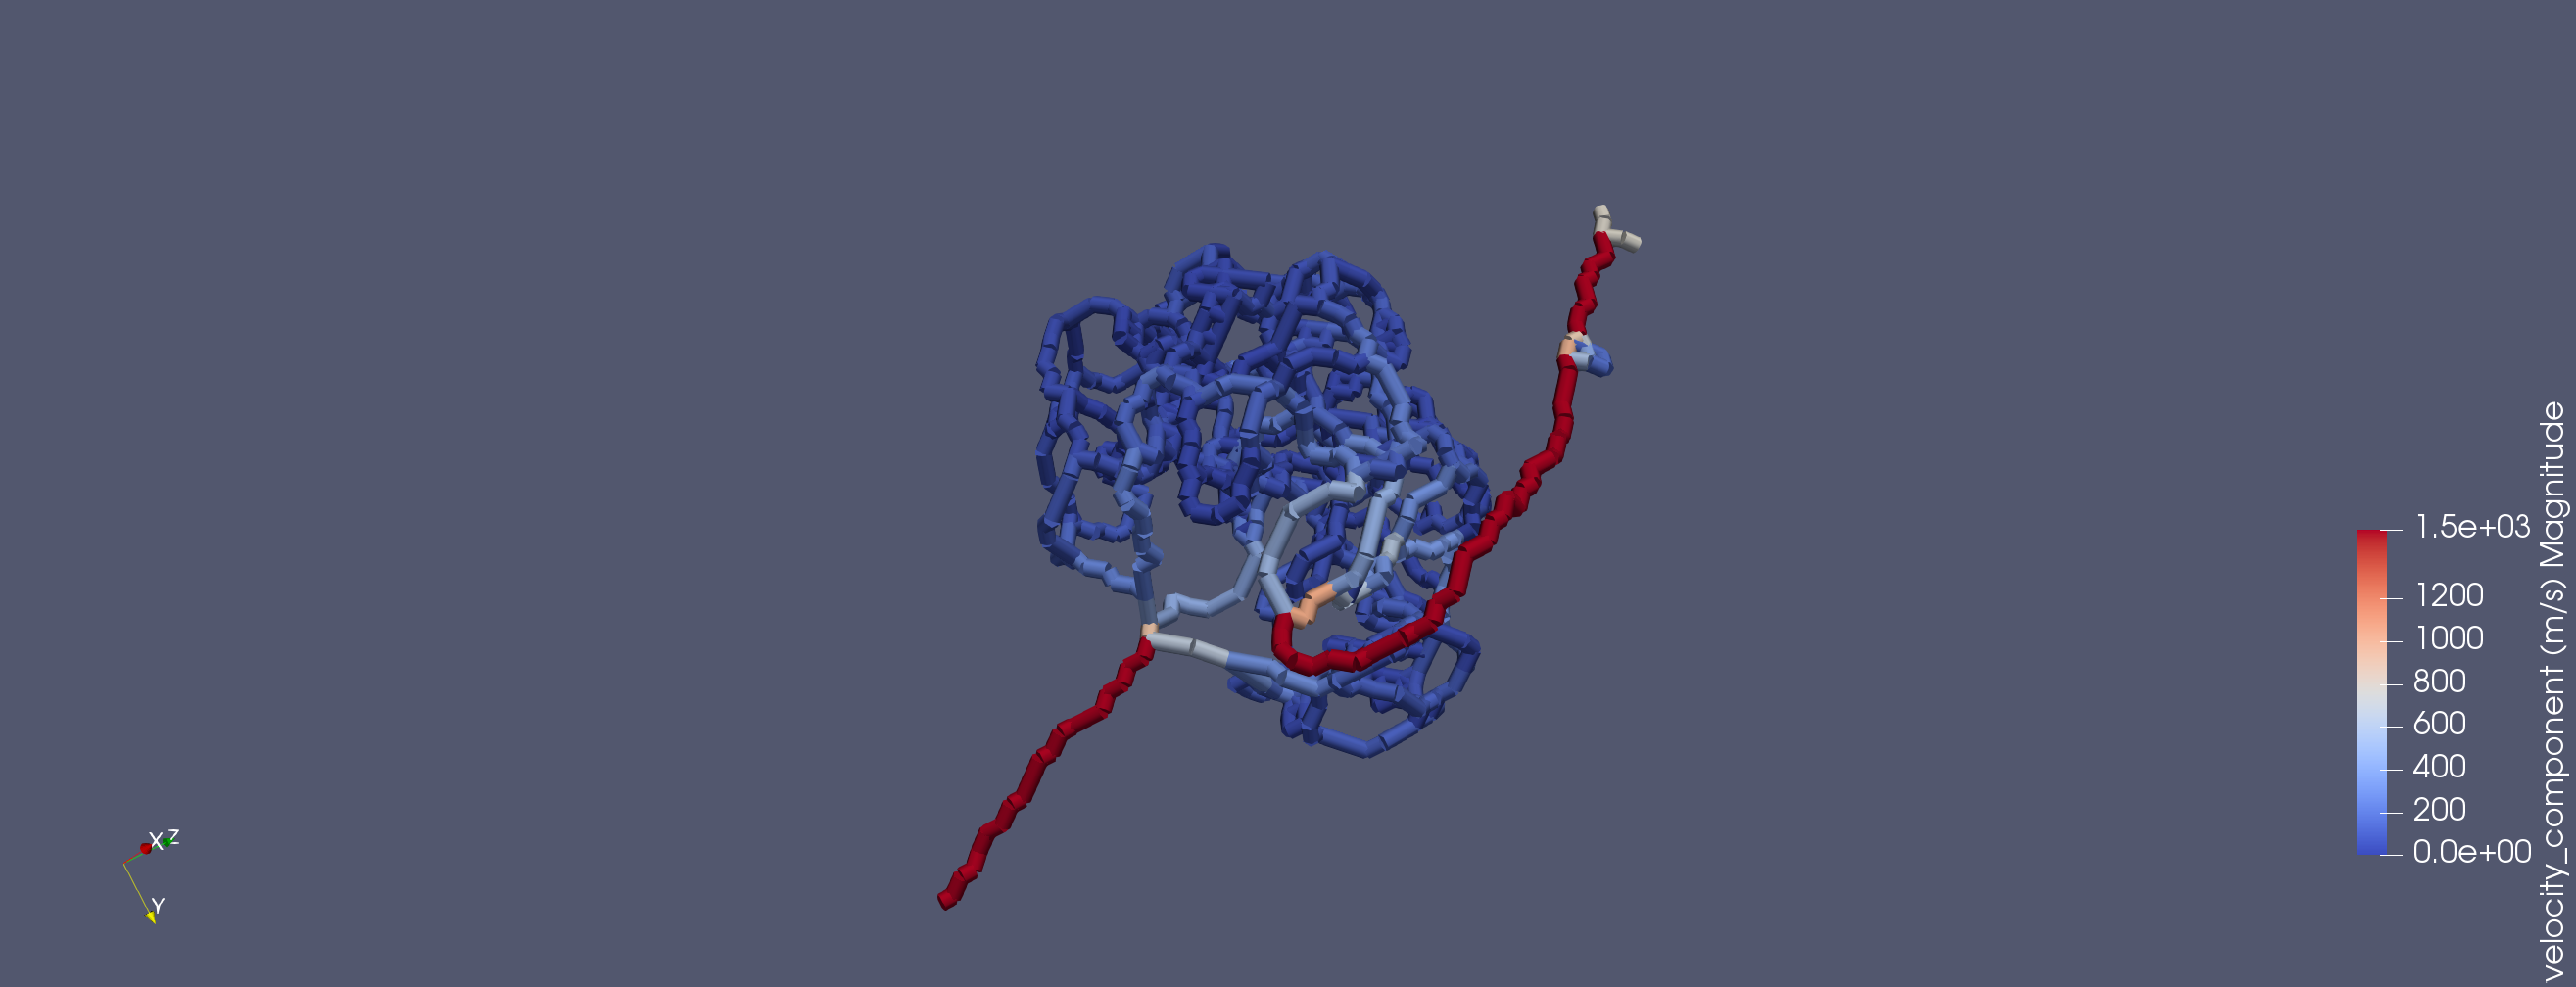
\includegraphics[height=62mm]{nephron_velocity}
\caption{Velocity Field in a Nephron}
\label{fig:nephron_velocity}
\end{figure}
Above is the result of a DuMuX 1p-1p blood flow simulation computed on a nephron network. The velocity field of the flow is visualized.\\

\begin{figure}[h]
\centering
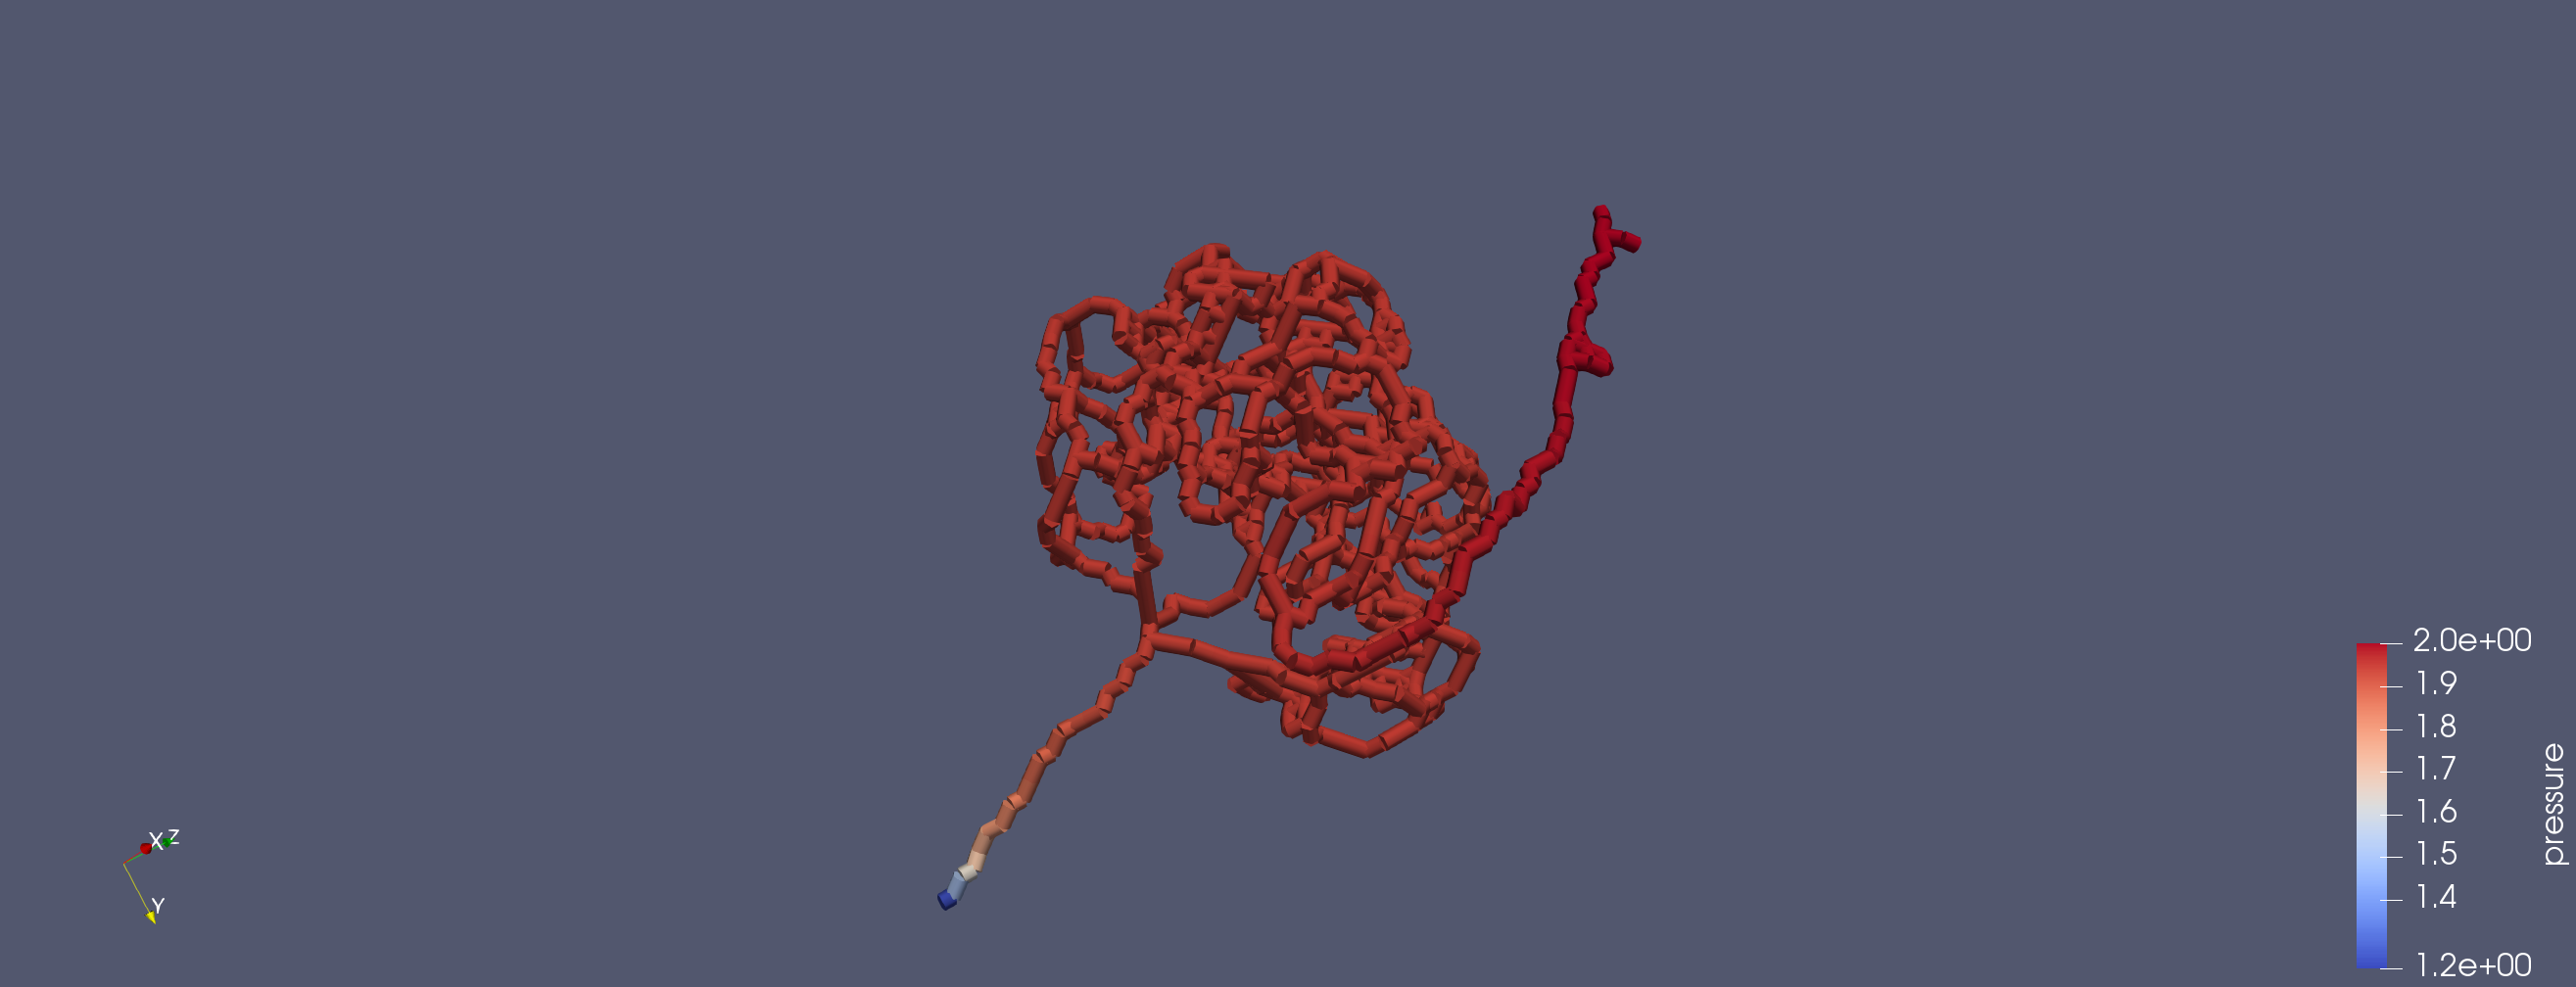
\includegraphics[height=62mm]{nephron_pressure}
\caption{Pressure Field in a Nephron}
\label{fig:nephron_pressure}
\end{figure}
Above is the result of a DuMuX 1p-1p blood flow simulation computed on a nephron network. The velocity field of the flow is visualized.\\

\subsection{Green's Function Code Results}
%Put all the extra plots etc. from Green's Function Code here.

Figure \ref{fig:Contour_Cardiac}  is the result of a Green's Method blood flow simulation computed on a Cardiac network. The Solute Concentration in the network is visualized.\\
\begin{figure}[h]
\centering
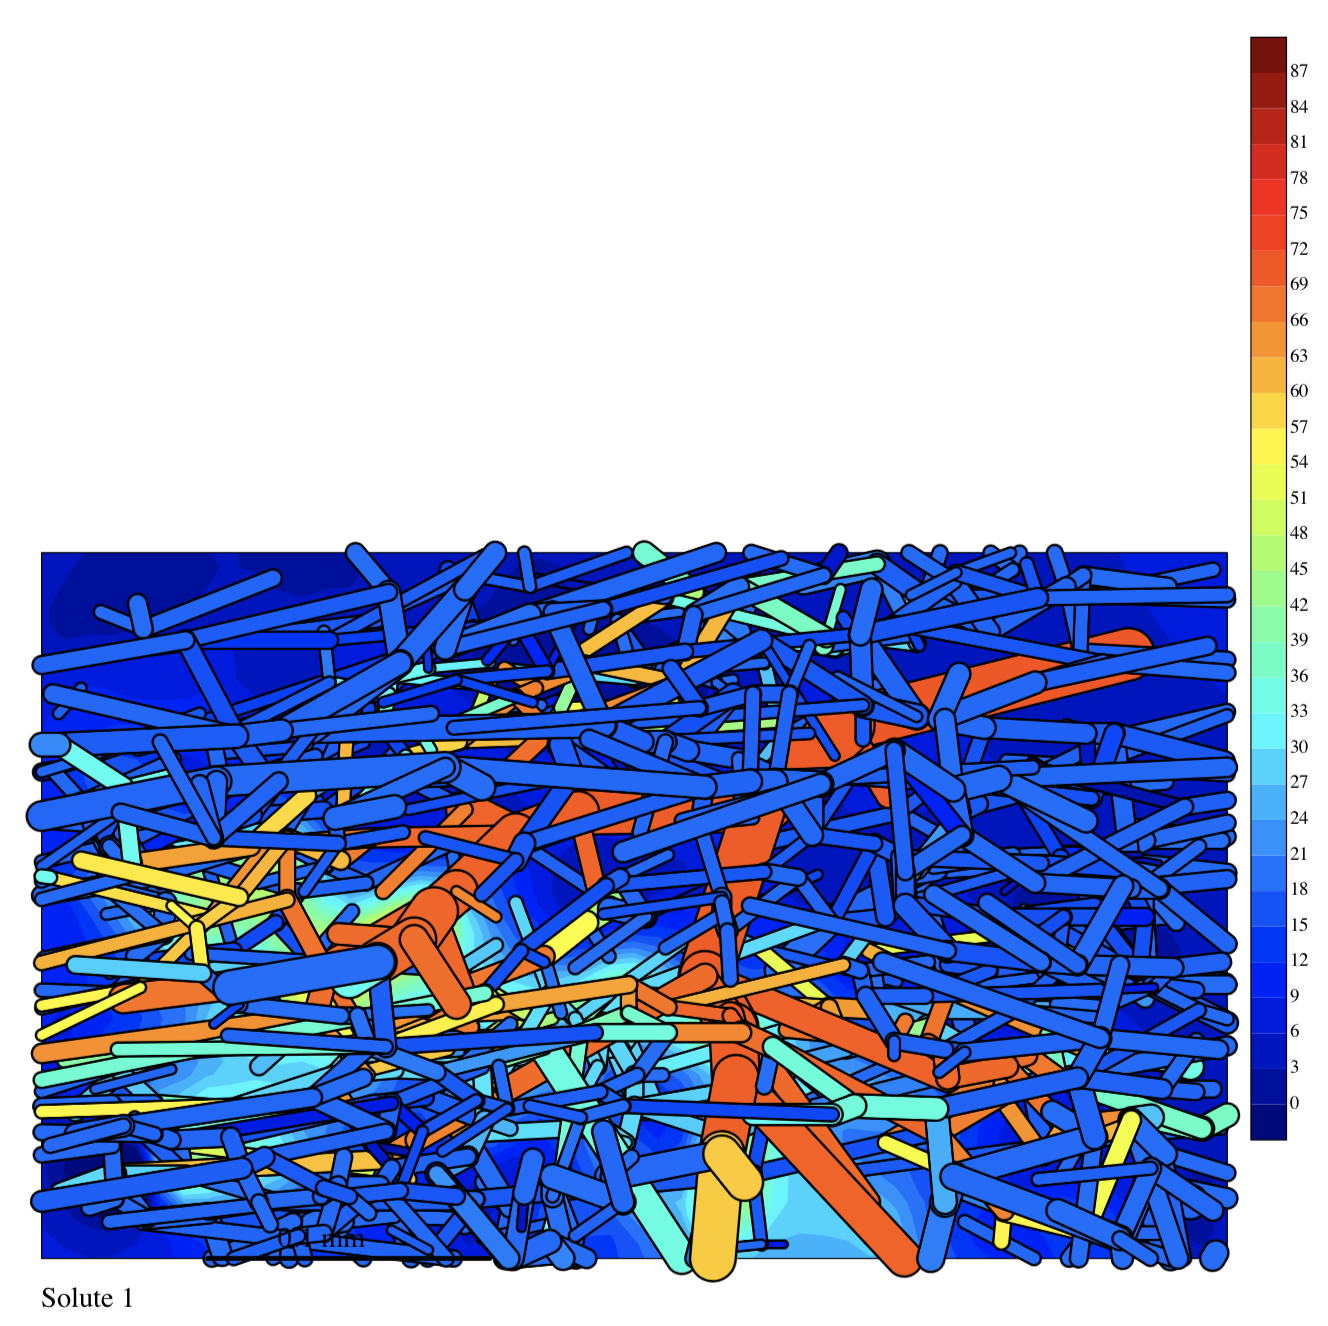
\includegraphics[width=170mm]{Contour_Cardiac}
\caption{Green's Contour Output for Cardiac Network}
\label{fig:Contour_Cardiac}
\end{figure}
%\section{Examples}
\label{s:Examples}

This appendix provides some additional hints and examples for the
layout and style of the thesis. It is worthwhile to look at the source
file \verb|Examples.tex| for this appendix to understand how it was
created.



\subsection{Tables}

Tables are left justified and the caption appears on top as seen in
Table~\ref{t:Translations}.

\begin{table}[ht]
\caption[Translations]{\label{t:Translations}Translations.}
\begin{tabular}{ll}
\hline
\textbf{English} & \textbf{German}\\
\hline
cell phone       & Handy\\
Diet Coke        & Coca Cola light\\
\hline
\end{tabular}
\end{table}



\subsection{Figures}

Figure~\ref{f:IRISlogo} shows a simple figure with a single picture
and Figure~\ref{f:SubfigureExample} shows a more complex figure
containing subfigures.

\begin{figure}[ht]
\centering

\includegraphics[width=.6\linewidth]{IRISlogo}
\caption[IRIS logo]{\label{f:IRISlogo}IRIS logo.}
\end{figure}

\begin{figure}[ht]
\centering
\subfigure[ETH logo]{
\includegraphics[height=12mm]{ETHlogo}}\quad
\subfigure[IRIS logo]{
\includegraphics[height=12mm]{IRISlogo}}
\caption[Subfigure example]{\label{f:SubfigureExample}Two pictures as
  part of a single figure through the magic of the subfigure package.}
\end{figure}



\subsection{Units}

The SIUnits package provides nice spacing for units as demonstrated in
Table~\ref{t:SIUnits}. Use of the package also makes it easy to change
the style or even the unit text in the future.

\begin{table}[ht]
\caption[Spacing for units]{\label{t:SIUnits}Spacing for units.}
\begin{tabular}{ll}
\hline
\textbf{Output}   & \textbf{Command}\\
\hline
42m               & \verb|42m|\\
\unit{42}{\metre} & \verb|\unit{42}{\metre}|\\
42 m              & \verb|42 m|\\
\hline
\end{tabular}
\end{table}



\subsection{Miscellany}

\begin{description}

\item[Capitalization.] When referring to a named table (such as in the
  previous section), the word \emph{table} is capitalized. The same is
  true for figures, chapters and sections.

\item[Naming of structural elements.] Refer to a \verb|\section| in
  \LaTeX\ as a chapter and call a \verb|\subsection| section. (I don't
  like the way \verb|\chapter|s are rendered in the report document
  class. Hence the suboptimal markup/naming correspondence.)

\item[Bibliography.] Use \verb|bibtex| to make your life easier and to
  produce consistently formatted entries.

\item[Contractions.] Avoid contractions. For instance, use ``do not''
  rather than ``don't.''

\item[Captions.] A brief version of a caption can be provided for the
  list of figures and tables as demonstrated with the caption of
  Figure~\ref{f:SubfigureExample}. The mechanism can also be used to
  get rid of the final period of a caption in the lists.

\end{description}



\end{document}
